\documentclass[twoside]{book}

% Packages required by doxygen
\usepackage{fixltx2e}
\usepackage{calc}
\usepackage{doxygen}
\usepackage[export]{adjustbox} % also loads graphicx
\usepackage{graphicx}
\usepackage[utf8]{inputenc}
\usepackage{makeidx}
\usepackage{multicol}
\usepackage{multirow}
\PassOptionsToPackage{warn}{textcomp}
\usepackage{textcomp}
\usepackage[nointegrals]{wasysym}
\usepackage[table]{xcolor}

% NLS support packages
Portuguese
% Font selection
\usepackage[T1]{fontenc}
\usepackage[scaled=.90]{helvet}
\usepackage{courier}
\usepackage{amssymb}
\usepackage{sectsty}
\renewcommand{\familydefault}{\sfdefault}
\allsectionsfont{%
  \fontseries{bc}\selectfont%
  \color{darkgray}%
}
\renewcommand{\DoxyLabelFont}{%
  \fontseries{bc}\selectfont%
  \color{darkgray}%
}
\newcommand{\+}{\discretionary{\mbox{\scriptsize$\hookleftarrow$}}{}{}}

% Page & text layout
\usepackage{geometry}
\geometry{%
  a4paper,%
  top=2.5cm,%
  bottom=2.5cm,%
  left=2.5cm,%
  right=2.5cm%
}
\tolerance=750
\hfuzz=15pt
\hbadness=750
\setlength{\emergencystretch}{15pt}
\setlength{\parindent}{0cm}
\setlength{\parskip}{0.2cm}
\makeatletter
\renewcommand{\paragraph}{%
  \@startsection{paragraph}{4}{0ex}{-1.0ex}{1.0ex}{%
    \normalfont\normalsize\bfseries\SS@parafont%
  }%
}
\renewcommand{\subparagraph}{%
  \@startsection{subparagraph}{5}{0ex}{-1.0ex}{1.0ex}{%
    \normalfont\normalsize\bfseries\SS@subparafont%
  }%
}
\makeatother

% Headers & footers
\usepackage{fancyhdr}
\pagestyle{fancyplain}
\fancyhead[LE]{\fancyplain{}{\bfseries\thepage}}
\fancyhead[CE]{\fancyplain{}{}}
\fancyhead[RE]{\fancyplain{}{\bfseries\leftmark}}
\fancyhead[LO]{\fancyplain{}{\bfseries\rightmark}}
\fancyhead[CO]{\fancyplain{}{}}
\fancyhead[RO]{\fancyplain{}{\bfseries\thepage}}
\fancyfoot[LE]{\fancyplain{}{}}
\fancyfoot[CE]{\fancyplain{}{}}
\fancyfoot[RE]{\fancyplain{}{\bfseries\scriptsize Gerado em Sábado, 31 de Outubro de 2015 20\+:10\+:20 para Software Ordem de serviço por Doxygen }}
\fancyfoot[LO]{\fancyplain{}{\bfseries\scriptsize Gerado em Sábado, 31 de Outubro de 2015 20\+:10\+:20 para Software Ordem de serviço por Doxygen }}
\fancyfoot[CO]{\fancyplain{}{}}
\fancyfoot[RO]{\fancyplain{}{}}
\renewcommand{\footrulewidth}{0.4pt}
\renewcommand{\chaptermark}[1]{%
  \markboth{#1}{}%
}
\renewcommand{\sectionmark}[1]{%
  \markright{\thesection\ #1}%
}

% Indices & bibliography
\usepackage{natbib}
\usepackage[titles]{tocloft}
\setcounter{tocdepth}{3}
\setcounter{secnumdepth}{5}
\makeindex

% Hyperlinks (required, but should be loaded last)
\usepackage{ifpdf}
\ifpdf
  \usepackage[pdftex,pagebackref=true]{hyperref}
\else
  \usepackage[ps2pdf,pagebackref=true]{hyperref}
\fi
\hypersetup{%
  colorlinks=true,%
  linkcolor=blue,%
  citecolor=blue,%
  unicode%
}

% Custom commands
\newcommand{\clearemptydoublepage}{%
  \newpage{\pagestyle{empty}\cleardoublepage}%
}


%===== C O N T E N T S =====

\begin{document}

% Titlepage & ToC
\hypersetup{pageanchor=false,
             bookmarks=true,
             bookmarksnumbered=true,
             pdfencoding=unicode
            }
\pagenumbering{roman}
\begin{titlepage}
\vspace*{7cm}
\begin{center}%
{\Large Software Ordem de serviço }\\
\vspace*{1cm}
{\large Gerado por Doxygen 1.8.10}\\
\vspace*{0.5cm}
{\small Sábado, 31 de Outubro de 2015 20:10:20}\\
\end{center}
\end{titlepage}
\clearemptydoublepage
\tableofcontents
\clearemptydoublepage
\pagenumbering{arabic}
\hypersetup{pageanchor=true}

%--- Begin generated contents ---
\chapter{Índice dos namespaces}
\section{Pacotes}
Lista de pacotes com uma breve descrição (se disponível)\+:\begin{DoxyCompactList}
\item\contentsline{section}{\hyperlink{namespace_controller}{Controller} }{\pageref{namespace_controller}}{}
\item\contentsline{section}{\hyperlink{namespace_model}{Model} }{\pageref{namespace_model}}{}
\item\contentsline{section}{\hyperlink{namespace_model_1_1_ordem__de___servico}{Model.\+Ordem\+\_\+de\+\_\+\+Servico} }{\pageref{namespace_model_1_1_ordem__de___servico}}{}
\item\contentsline{section}{\hyperlink{namespace_model_1_1_pessoa__e___usuario}{Model.\+Pessoa\+\_\+e\+\_\+\+Usuario} }{\pageref{namespace_model_1_1_pessoa__e___usuario}}{}
\item\contentsline{section}{\hyperlink{namespace_view}{View} }{\pageref{namespace_view}}{}
\item\contentsline{section}{\hyperlink{namespace_view_1_1_formularios___usuarios}{View.\+Formularios\+\_\+\+Usuarios} }{\pageref{namespace_view_1_1_formularios___usuarios}}{}
\item\contentsline{section}{\hyperlink{namespace_view_1_1_opicoes}{View.\+Opicoes} }{\pageref{namespace_view_1_1_opicoes}}{}
\item\contentsline{section}{\hyperlink{namespace_view_1_1_o_s}{View.\+O\+S} }{\pageref{namespace_view_1_1_o_s}}{}
\item\contentsline{section}{\hyperlink{namespace_view_1_1_outros}{View.\+Outros} }{\pageref{namespace_view_1_1_outros}}{}
\item\contentsline{section}{\hyperlink{namespace_view_1_1_pessoas}{View.\+Pessoas} }{\pageref{namespace_view_1_1_pessoas}}{}
\item\contentsline{section}{\hyperlink{namespace_view_1_1_properties}{View.\+Properties} }{\pageref{namespace_view_1_1_properties}}{}
\item\contentsline{section}{\hyperlink{namespace_view_1_1_servicos}{View.\+Servicos} }{\pageref{namespace_view_1_1_servicos}}{}
\item\contentsline{section}{\hyperlink{namespace_view_1_1_usuario}{View.\+Usuario} }{\pageref{namespace_view_1_1_usuario}}{}
\end{DoxyCompactList}

\chapter{Índice da hierarquia}
\section{Hierarquia de classes}
Esta lista de heranças está organizada, dentro do possível, por ordem alfabética\+:\begin{DoxyCompactList}
\item \contentsline{section}{Model.\+Backup}{\pageref{class_model_1_1_backup}}{}
\item \contentsline{section}{Model.\+Empresa}{\pageref{class_model_1_1_empresa}}{}
\item Form\begin{DoxyCompactList}
\item \contentsline{section}{View.\+Formularios\+\_\+\+Usuarios.\+Frm\+\_\+\+New\+Usu}{\pageref{class_view_1_1_formularios___usuarios_1_1_frm___new_usu}}{}
\item \contentsline{section}{View.\+Frm\+\_\+\+Backup}{\pageref{class_view_1_1_frm___backup}}{}
\item \contentsline{section}{View.\+Frm\+\_\+\+Imprimir\+O\+S}{\pageref{class_view_1_1_frm___imprimir_o_s}}{}
\item \contentsline{section}{View.\+Frm\+\_\+\+Login}{\pageref{class_view_1_1_frm___login}}{}
\item \contentsline{section}{View.\+Frm\+\_\+\+Pai}{\pageref{class_view_1_1_frm___pai}}{}
\item \contentsline{section}{View.\+Opicoes.\+Frm\+\_\+\+Opicoes\+Inicial}{\pageref{class_view_1_1_opicoes_1_1_frm___opicoes_inicial}}{}
\item \contentsline{section}{View.\+O\+S.\+Frm\+\_\+\+Editar\+O\+S}{\pageref{class_view_1_1_o_s_1_1_frm___editar_o_s}}{}
\item \contentsline{section}{View.\+O\+S.\+Frm\+\_\+\+Listar\+O\+S}{\pageref{class_view_1_1_o_s_1_1_frm___listar_o_s}}{}
\item \contentsline{section}{View.\+O\+S.\+Frm\+\_\+\+New\+Ordem}{\pageref{class_view_1_1_o_s_1_1_frm___new_ordem}}{}
\item \contentsline{section}{View.\+Outros.\+Frm\+\_\+\+Sobre}{\pageref{class_view_1_1_outros_1_1_frm___sobre}}{}
\item \contentsline{section}{View.\+Pessoas.\+Frm\+\_\+\+Listar\+Fisica}{\pageref{class_view_1_1_pessoas_1_1_frm___listar_fisica}}{}
\item \contentsline{section}{View.\+Pessoas.\+Frm\+\_\+\+Listar\+Juridica}{\pageref{class_view_1_1_pessoas_1_1_frm___listar_juridica}}{}
\item \contentsline{section}{View.\+Pessoas.\+Frm\+\_\+\+Pessoa\+Fisica}{\pageref{class_view_1_1_pessoas_1_1_frm___pessoa_fisica}}{}
\item \contentsline{section}{View.\+Pessoas.\+Frm\+\_\+\+Pessoa\+Juridica}{\pageref{class_view_1_1_pessoas_1_1_frm___pessoa_juridica}}{}
\item \contentsline{section}{View.\+Usuario.\+Frm\+\_\+\+Edit\+Usu}{\pageref{class_view_1_1_usuario_1_1_frm___edit_usu}}{}
\item \contentsline{section}{View.\+Usuario.\+Frm\+\_\+\+Listar\+Usuarios}{\pageref{class_view_1_1_usuario_1_1_frm___listar_usuarios}}{}
\end{DoxyCompactList}
\item \contentsline{section}{Model.\+Ordem\+\_\+de\+\_\+\+Servico.\+Ordem\+Servico}{\pageref{class_model_1_1_ordem__de___servico_1_1_ordem_servico}}{}
\item \contentsline{section}{Model.\+Pessoa\+\_\+e\+\_\+\+Usuario.\+Pessoa}{\pageref{class_model_1_1_pessoa__e___usuario_1_1_pessoa}}{}
\begin{DoxyCompactList}
\item \contentsline{section}{Model.\+Pessoa\+\_\+e\+\_\+\+Usuario.\+Fisica}{\pageref{class_model_1_1_pessoa__e___usuario_1_1_fisica}}{}
\item \contentsline{section}{Model.\+Pessoa\+\_\+e\+\_\+\+Usuario.\+Juridica}{\pageref{class_model_1_1_pessoa__e___usuario_1_1_juridica}}{}
\end{DoxyCompactList}
\item \contentsline{section}{View\+Console.\+Program}{\pageref{class_view_console_1_1_program}}{}
\item \contentsline{section}{Model.\+Ordem\+\_\+de\+\_\+\+Servico.\+Servico}{\pageref{class_model_1_1_ordem__de___servico_1_1_servico}}{}
\item \contentsline{section}{Model.\+Pessoa\+\_\+e\+\_\+\+Usuario.\+Usuario}{\pageref{class_model_1_1_pessoa__e___usuario_1_1_usuario}}{}
\end{DoxyCompactList}

\chapter{Índice dos componentes}
\section{Lista de componentes}
Lista de classes, estruturas, uniões e interfaces com uma breve descrição\+:\begin{DoxyCompactList}
\item\contentsline{section}{\hyperlink{class_controller_1_1_controller_backup}{Controller.\+Controller\+Backup} }{\pageref{class_controller_1_1_controller_backup}}{}
\item\contentsline{section}{\hyperlink{class_controller_1_1_controller_email}{Controller.\+Controller\+Email} }{\pageref{class_controller_1_1_controller_email}}{}
\item\contentsline{section}{\hyperlink{class_controller_1_1_controller_empresa}{Controller.\+Controller\+Empresa} }{\pageref{class_controller_1_1_controller_empresa}}{}
\item\contentsline{section}{\hyperlink{class_controller_1_1_controller_fisica}{Controller.\+Controller\+Fisica} }{\pageref{class_controller_1_1_controller_fisica}}{}
\item\contentsline{section}{\hyperlink{class_controller_1_1_controller_juridica}{Controller.\+Controller\+Juridica} }{\pageref{class_controller_1_1_controller_juridica}}{}
\item\contentsline{section}{\hyperlink{class_controller_1_1_controller_ordem_servico}{Controller.\+Controller\+Ordem\+Servico} }{\pageref{class_controller_1_1_controller_ordem_servico}}{}
\item\contentsline{section}{\hyperlink{class_controller_1_1_controller_servico}{Controller.\+Controller\+Servico} }{\pageref{class_controller_1_1_controller_servico}}{}
\item\contentsline{section}{\hyperlink{class_controller_1_1_controller_servico_base}{Controller.\+Controller\+Servico\+Base} }{\pageref{class_controller_1_1_controller_servico_base}}{}
\item\contentsline{section}{\hyperlink{class_controller_1_1_controller_usuario}{Controller.\+Controller\+Usuario} \\*Usada como classe dos técnicos da empresa, cada um com o seu login. }{\pageref{class_controller_1_1_controller_usuario}}{}
\item\contentsline{section}{\hyperlink{class_model_1_1_email}{Model.\+Email} }{\pageref{class_model_1_1_email}}{}
\item\contentsline{section}{\hyperlink{class_model_1_1_empresa}{Model.\+Empresa} }{\pageref{class_model_1_1_empresa}}{}
\item\contentsline{section}{\hyperlink{class_model_1_1_pessoa__e___usuario_1_1_fisica}{Model.\+Pessoa\+\_\+e\+\_\+\+Usuario.\+Fisica} }{\pageref{class_model_1_1_pessoa__e___usuario_1_1_fisica}}{}
\item\contentsline{section}{\hyperlink{class_view_1_1_frm___backup}{View.\+Frm\+\_\+\+Backup} }{\pageref{class_view_1_1_frm___backup}}{}
\item\contentsline{section}{\hyperlink{class_view_1_1_frm___config_email}{View.\+Frm\+\_\+\+Config\+Email} }{\pageref{class_view_1_1_frm___config_email}}{}
\item\contentsline{section}{\hyperlink{class_view_1_1_o_s_1_1_frm___editar_o_s}{View.\+O\+S.\+Frm\+\_\+\+Editar\+O\+S} }{\pageref{class_view_1_1_o_s_1_1_frm___editar_o_s}}{}
\item\contentsline{section}{\hyperlink{class_view_1_1_frm___editar_servico_base}{View.\+Frm\+\_\+\+Editar\+Servico\+Base} }{\pageref{class_view_1_1_frm___editar_servico_base}}{}
\item\contentsline{section}{\hyperlink{class_view_1_1_usuario_1_1_frm___edit_usu}{View.\+Usuario.\+Frm\+\_\+\+Edit\+Usu} }{\pageref{class_view_1_1_usuario_1_1_frm___edit_usu}}{}
\item\contentsline{section}{\hyperlink{class_view_1_1_frm___email_base}{View.\+Frm\+\_\+\+Email\+Base} }{\pageref{class_view_1_1_frm___email_base}}{}
\item\contentsline{section}{\hyperlink{class_view_1_1_o_s_1_1_frm___excluir_o_s}{View.\+O\+S.\+Frm\+\_\+\+Excluir\+O\+S} }{\pageref{class_view_1_1_o_s_1_1_frm___excluir_o_s}}{}
\item\contentsline{section}{\hyperlink{class_view_1_1_pessoas_1_1_frm___excluir_pessoa_fisica}{View.\+Pessoas.\+Frm\+\_\+\+Excluir\+Pessoa\+Fisica} }{\pageref{class_view_1_1_pessoas_1_1_frm___excluir_pessoa_fisica}}{}
\item\contentsline{section}{\hyperlink{class_view_1_1_pessoas_1_1_frm___excluir_pessoa_juridica}{View.\+Pessoas.\+Frm\+\_\+\+Excluir\+Pessoa\+Juridica} }{\pageref{class_view_1_1_pessoas_1_1_frm___excluir_pessoa_juridica}}{}
\item\contentsline{section}{\hyperlink{class_view_1_1_servicos_1_1_frm___excluir_servico}{View.\+Servicos.\+Frm\+\_\+\+Excluir\+Servico} }{\pageref{class_view_1_1_servicos_1_1_frm___excluir_servico}}{}
\item\contentsline{section}{\hyperlink{class_view_1_1_usuario_1_1_frm___excluir_usuario}{View.\+Usuario.\+Frm\+\_\+\+Excluir\+Usuario} }{\pageref{class_view_1_1_usuario_1_1_frm___excluir_usuario}}{}
\item\contentsline{section}{\hyperlink{class_view_1_1_frm___imprimir_o_s}{View.\+Frm\+\_\+\+Imprimir\+O\+S} }{\pageref{class_view_1_1_frm___imprimir_o_s}}{}
\item\contentsline{section}{\hyperlink{class_view_1_1_pessoas_1_1_frm___listar_fisica}{View.\+Pessoas.\+Frm\+\_\+\+Listar\+Fisica} }{\pageref{class_view_1_1_pessoas_1_1_frm___listar_fisica}}{}
\item\contentsline{section}{\hyperlink{class_view_1_1_pessoas_1_1_frm___listar_juridica}{View.\+Pessoas.\+Frm\+\_\+\+Listar\+Juridica} }{\pageref{class_view_1_1_pessoas_1_1_frm___listar_juridica}}{}
\item\contentsline{section}{\hyperlink{class_view_1_1_o_s_1_1_frm___listar_o_s}{View.\+O\+S.\+Frm\+\_\+\+Listar\+O\+S} }{\pageref{class_view_1_1_o_s_1_1_frm___listar_o_s}}{}
\item\contentsline{section}{\hyperlink{class_view_1_1_frm___listar_servico}{View.\+Frm\+\_\+\+Listar\+Servico} }{\pageref{class_view_1_1_frm___listar_servico}}{}
\item\contentsline{section}{\hyperlink{class_view_1_1_frm___listar_servico_base}{View.\+Frm\+\_\+\+Listar\+Servico\+Base} }{\pageref{class_view_1_1_frm___listar_servico_base}}{}
\item\contentsline{section}{\hyperlink{class_view_1_1_usuario_1_1_frm___listar_usuarios}{View.\+Usuario.\+Frm\+\_\+\+Listar\+Usuarios} }{\pageref{class_view_1_1_usuario_1_1_frm___listar_usuarios}}{}
\item\contentsline{section}{\hyperlink{class_view_1_1_frm___login}{View.\+Frm\+\_\+\+Login} }{\pageref{class_view_1_1_frm___login}}{}
\item\contentsline{section}{\hyperlink{class_view_1_1_o_s_1_1_frm___new_ordem}{View.\+O\+S.\+Frm\+\_\+\+New\+Ordem} }{\pageref{class_view_1_1_o_s_1_1_frm___new_ordem}}{}
\item\contentsline{section}{\hyperlink{class_view_1_1_frm___new_servico_base}{View.\+Frm\+\_\+\+New\+Servico\+Base} }{\pageref{class_view_1_1_frm___new_servico_base}}{}
\item\contentsline{section}{\hyperlink{class_view_1_1_formularios___usuarios_1_1_frm___new_usu}{View.\+Formularios\+\_\+\+Usuarios.\+Frm\+\_\+\+New\+Usu} }{\pageref{class_view_1_1_formularios___usuarios_1_1_frm___new_usu}}{}
\item\contentsline{section}{\hyperlink{class_view_1_1_opicoes_1_1_frm___opicoes_inicial}{View.\+Opicoes.\+Frm\+\_\+\+Opicoes\+Inicial} }{\pageref{class_view_1_1_opicoes_1_1_frm___opicoes_inicial}}{}
\item\contentsline{section}{\hyperlink{class_view_1_1_frm___pai}{View.\+Frm\+\_\+\+Pai} }{\pageref{class_view_1_1_frm___pai}}{}
\item\contentsline{section}{\hyperlink{class_view_1_1_pessoas_1_1_frm___pessoa_fisica}{View.\+Pessoas.\+Frm\+\_\+\+Pessoa\+Fisica} }{\pageref{class_view_1_1_pessoas_1_1_frm___pessoa_fisica}}{}
\item\contentsline{section}{\hyperlink{class_view_1_1_pessoas_1_1_frm___pessoa_juridica}{View.\+Pessoas.\+Frm\+\_\+\+Pessoa\+Juridica} }{\pageref{class_view_1_1_pessoas_1_1_frm___pessoa_juridica}}{}
\item\contentsline{section}{\hyperlink{class_view_1_1_frm___servico}{View.\+Frm\+\_\+\+Servico} }{\pageref{class_view_1_1_frm___servico}}{}
\item\contentsline{section}{\hyperlink{class_view_1_1_outros_1_1_frm___sobre}{View.\+Outros.\+Frm\+\_\+\+Sobre} }{\pageref{class_view_1_1_outros_1_1_frm___sobre}}{}
\item\contentsline{section}{\hyperlink{class_model_1_1_pessoa__e___usuario_1_1_juridica}{Model.\+Pessoa\+\_\+e\+\_\+\+Usuario.\+Juridica} }{\pageref{class_model_1_1_pessoa__e___usuario_1_1_juridica}}{}
\item\contentsline{section}{\hyperlink{class_model_1_1_ordem__de___servico_1_1_ordem_servico}{Model.\+Ordem\+\_\+de\+\_\+\+Servico.\+Ordem\+Servico} }{\pageref{class_model_1_1_ordem__de___servico_1_1_ordem_servico}}{}
\item\contentsline{section}{\hyperlink{class_model_1_1_pessoa__e___usuario_1_1_pessoa}{Model.\+Pessoa\+\_\+e\+\_\+\+Usuario.\+Pessoa} }{\pageref{class_model_1_1_pessoa__e___usuario_1_1_pessoa}}{}
\item\contentsline{section}{\hyperlink{class_model_1_1_ordem__de___servico_1_1_servico}{Model.\+Ordem\+\_\+de\+\_\+\+Servico.\+Servico} }{\pageref{class_model_1_1_ordem__de___servico_1_1_servico}}{}
\item\contentsline{section}{\hyperlink{class_model_1_1_servico_base}{Model.\+Servico\+Base} }{\pageref{class_model_1_1_servico_base}}{}
\item\contentsline{section}{\hyperlink{class_model_1_1_pessoa__e___usuario_1_1_usuario}{Model.\+Pessoa\+\_\+e\+\_\+\+Usuario.\+Usuario} }{\pageref{class_model_1_1_pessoa__e___usuario_1_1_usuario}}{}
\end{DoxyCompactList}

\chapter{Documentação dos namespaces}
\hypertarget{namespace_model}{}\section{Referência ao namespace Model}
\label{namespace_model}\index{Model@{Model}}
\subsection*{Namespaces}
\begin{DoxyCompactItemize}
\item 
namespace \hyperlink{namespace_model_1_1_ordem__de___servico}{Ordem\+\_\+de\+\_\+\+Servico}
\item 
namespace \hyperlink{namespace_model_1_1_pessoa__e___usuario}{Pessoa\+\_\+e\+\_\+\+Usuario}
\end{DoxyCompactItemize}
\subsection*{Componentes}
\begin{DoxyCompactItemize}
\item 
class \hyperlink{class_model_1_1_email}{Email}
\item 
class \hyperlink{class_model_1_1_empresa}{Empresa}
\item 
class \hyperlink{class_model_1_1_servico_base}{Servico\+Base}
\end{DoxyCompactItemize}

\hypertarget{namespace_model_1_1_ordem__de___servico}{}\section{Referência ao namespace Model.\+Ordem\+\_\+de\+\_\+\+Servico}
\label{namespace_model_1_1_ordem__de___servico}\index{Model.\+Ordem\+\_\+de\+\_\+\+Servico@{Model.\+Ordem\+\_\+de\+\_\+\+Servico}}
\subsection*{Componentes}
\begin{DoxyCompactItemize}
\item 
class \hyperlink{class_model_1_1_ordem__de___servico_1_1_ordem_servico}{Ordem\+Servico}
\item 
class \hyperlink{class_model_1_1_ordem__de___servico_1_1_servico}{Servico}
\end{DoxyCompactItemize}

\hypertarget{namespace_model_1_1_pessoa__e___usuario}{}\section{Referência ao namespace Model.\+Pessoa\+\_\+e\+\_\+\+Usuario}
\label{namespace_model_1_1_pessoa__e___usuario}\index{Model.\+Pessoa\+\_\+e\+\_\+\+Usuario@{Model.\+Pessoa\+\_\+e\+\_\+\+Usuario}}
\subsection*{Componentes}
\begin{DoxyCompactItemize}
\item 
class \hyperlink{class_model_1_1_pessoa__e___usuario_1_1_fisica}{Fisica}
\item 
class \hyperlink{class_model_1_1_pessoa__e___usuario_1_1_juridica}{Juridica}
\item 
class \hyperlink{class_model_1_1_pessoa__e___usuario_1_1_pessoa}{Pessoa}
\item 
class \hyperlink{class_model_1_1_pessoa__e___usuario_1_1_usuario}{Usuario}
\end{DoxyCompactItemize}

\hypertarget{namespace_view}{}\section{Referência ao namespace View}
\label{namespace_view}\index{View@{View}}
\subsection*{Namespaces}
\begin{DoxyCompactItemize}
\item 
namespace \hyperlink{namespace_view_1_1_formularios___usuarios}{Formularios\+\_\+\+Usuarios}
\item 
namespace \hyperlink{namespace_view_1_1_opicoes}{Opicoes}
\item 
namespace \hyperlink{namespace_view_1_1_o_s}{O\+S}
\item 
namespace \hyperlink{namespace_view_1_1_outros}{Outros}
\item 
namespace \hyperlink{namespace_view_1_1_pessoas}{Pessoas}
\item 
namespace \hyperlink{namespace_view_1_1_properties}{Properties}
\item 
namespace \hyperlink{namespace_view_1_1_usuario}{Usuario}
\end{DoxyCompactItemize}
\subsection*{Componentes}
\begin{DoxyCompactItemize}
\item 
class \hyperlink{class_view_1_1_frm___backup}{Frm\+\_\+\+Backup}
\item 
class \hyperlink{class_view_1_1_frm___imprimir_o_s}{Frm\+\_\+\+Imprimir\+O\+S}
\item 
class \hyperlink{class_view_1_1_frm___login}{Frm\+\_\+\+Login}
\item 
class \hyperlink{class_view_1_1_frm___pai}{Frm\+\_\+\+Pai}
\item 
class {\bfseries Program}
\end{DoxyCompactItemize}

\hypertarget{namespace_view_1_1_formularios___usuarios}{}\section{Referência ao namespace View.\+Formularios\+\_\+\+Usuarios}
\label{namespace_view_1_1_formularios___usuarios}\index{View.\+Formularios\+\_\+\+Usuarios@{View.\+Formularios\+\_\+\+Usuarios}}
\subsection*{Componentes}
\begin{DoxyCompactItemize}
\item 
class \hyperlink{class_view_1_1_formularios___usuarios_1_1_frm___new_usu}{Frm\+\_\+\+New\+Usu}
\end{DoxyCompactItemize}

\hypertarget{namespace_view_1_1_opicoes}{}\section{Referência ao namespace View.\+Opicoes}
\label{namespace_view_1_1_opicoes}\index{View.\+Opicoes@{View.\+Opicoes}}
\subsection*{Componentes}
\begin{DoxyCompactItemize}
\item 
class \hyperlink{class_view_1_1_opicoes_1_1_frm___opicoes_inicial}{Frm\+\_\+\+Opicoes\+Inicial}
\end{DoxyCompactItemize}

\hypertarget{namespace_view_1_1_o_s}{}\section{Referência ao namespace View.\+O\+S}
\label{namespace_view_1_1_o_s}\index{View.\+O\+S@{View.\+O\+S}}
\subsection*{Componentes}
\begin{DoxyCompactItemize}
\item 
class \hyperlink{class_view_1_1_o_s_1_1_frm___editar_o_s}{Frm\+\_\+\+Editar\+O\+S}
\item 
class \hyperlink{class_view_1_1_o_s_1_1_frm___listar_o_s}{Frm\+\_\+\+Listar\+O\+S}
\item 
class \hyperlink{class_view_1_1_o_s_1_1_frm___new_ordem}{Frm\+\_\+\+New\+Ordem}
\end{DoxyCompactItemize}

\hypertarget{namespace_view_1_1_outros}{}\section{Referência ao namespace View.\+Outros}
\label{namespace_view_1_1_outros}\index{View.\+Outros@{View.\+Outros}}
\subsection*{Componentes}
\begin{DoxyCompactItemize}
\item 
class \hyperlink{class_view_1_1_outros_1_1_frm___sobre}{Frm\+\_\+\+Sobre}
\end{DoxyCompactItemize}

\hypertarget{namespace_view_1_1_pessoas}{}\section{Referência ao namespace View.\+Pessoas}
\label{namespace_view_1_1_pessoas}\index{View.\+Pessoas@{View.\+Pessoas}}
\subsection*{Componentes}
\begin{DoxyCompactItemize}
\item 
class \hyperlink{class_view_1_1_pessoas_1_1_frm___listar_fisica}{Frm\+\_\+\+Listar\+Fisica}
\item 
class \hyperlink{class_view_1_1_pessoas_1_1_frm___listar_juridica}{Frm\+\_\+\+Listar\+Juridica}
\item 
class \hyperlink{class_view_1_1_pessoas_1_1_frm___pessoa_fisica}{Frm\+\_\+\+Pessoa\+Fisica}
\item 
class \hyperlink{class_view_1_1_pessoas_1_1_frm___pessoa_juridica}{Frm\+\_\+\+Pessoa\+Juridica}
\end{DoxyCompactItemize}

\hypertarget{namespace_view_1_1_properties}{}\section{Referência ao namespace View.\+Properties}
\label{namespace_view_1_1_properties}\index{View.\+Properties@{View.\+Properties}}
\subsection*{Componentes}
\begin{DoxyCompactItemize}
\item 
class {\bfseries Resources}
\begin{DoxyCompactList}\small\item\em Uma classe de recurso de tipo de alta segurança, para pesquisar cadeias de caracteres localizadas etc. \end{DoxyCompactList}\item 
class {\bfseries Settings}
\end{DoxyCompactItemize}

\hypertarget{namespace_view_1_1_usuario}{}\section{Referência ao namespace View.\+Usuario}
\label{namespace_view_1_1_usuario}\index{View.\+Usuario@{View.\+Usuario}}
\subsection*{Componentes}
\begin{DoxyCompactItemize}
\item 
class \hyperlink{class_view_1_1_usuario_1_1_frm___edit_usu}{Frm\+\_\+\+Edit\+Usu}
\item 
class \hyperlink{class_view_1_1_usuario_1_1_frm___excluir_usuario}{Frm\+\_\+\+Excluir\+Usuario}
\item 
class \hyperlink{class_view_1_1_usuario_1_1_frm___listar_usuarios}{Frm\+\_\+\+Listar\+Usuarios}
\end{DoxyCompactItemize}

\hypertarget{namespace_view_console}{}\section{Referência ao namespace View\+Console}
\label{namespace_view_console}\index{View\+Console@{View\+Console}}
\subsection*{Componentes}
\begin{DoxyCompactItemize}
\item 
class {\bfseries Menu\+Principal}
\item 
class {\bfseries Ordem\+De\+Servico}
\item 
class {\bfseries Pessoa\+Fisica}
\item 
class {\bfseries Pessoa\+Juridica}
\item 
class \hyperlink{class_view_console_1_1_program}{Program}
\end{DoxyCompactItemize}

\chapter{Documentação da classe}
\hypertarget{class_model_1_1_backup}{}\section{Referência à classe Model.\+Backup}
\label{class_model_1_1_backup}\index{Model.\+Backup@{Model.\+Backup}}
\subsection*{Membros públicos}
\begin{DoxyCompactItemize}
\item 
void \hyperlink{class_model_1_1_backup_a174d26d6d0ea5375a66d3e09d2b25ce9}{Criar\+Arquivo\+Zip} (List$<$ string $>$ arquivos, string Arquivo\+Destino)
\begin{DoxyCompactList}\small\item\em Criando arquivo \char`\"{}\+Zip\char`\"{} de backup das informações. \end{DoxyCompactList}\item 
void \hyperlink{class_model_1_1_backup_adb275145c087e858eba8661f1a026108}{Extrair\+Arquivo\+Zip} (string localizacao\+Arquivo\+Zip, string destino)
\begin{DoxyCompactList}\small\item\em Extraindo informações do \char`\"{}\+Zip\char`\"{} e colocando na pasta do software. \end{DoxyCompactList}\end{DoxyCompactItemize}


\subsection{Documentação dos métodos}
\hypertarget{class_model_1_1_backup_a174d26d6d0ea5375a66d3e09d2b25ce9}{}\index{Model\+::\+Backup@{Model\+::\+Backup}!Criar\+Arquivo\+Zip@{Criar\+Arquivo\+Zip}}
\index{Criar\+Arquivo\+Zip@{Criar\+Arquivo\+Zip}!Model\+::\+Backup@{Model\+::\+Backup}}
\subsubsection[{Criar\+Arquivo\+Zip(\+List$<$ string $>$ arquivos, string Arquivo\+Destino)}]{\setlength{\rightskip}{0pt plus 5cm}void Model.\+Backup.\+Criar\+Arquivo\+Zip (
\begin{DoxyParamCaption}
\item[{List$<$ string $>$}]{arquivos, }
\item[{string}]{Arquivo\+Destino}
\end{DoxyParamCaption}
)}\label{class_model_1_1_backup_a174d26d6d0ea5375a66d3e09d2b25ce9}


Criando arquivo \char`\"{}\+Zip\char`\"{} de backup das informações. 


\begin{DoxyParams}{Parâmetros}
{\em arquivos} & \\
\hline
{\em Arquivo\+Destino} & \\
\hline
\end{DoxyParams}
\hypertarget{class_model_1_1_backup_adb275145c087e858eba8661f1a026108}{}\index{Model\+::\+Backup@{Model\+::\+Backup}!Extrair\+Arquivo\+Zip@{Extrair\+Arquivo\+Zip}}
\index{Extrair\+Arquivo\+Zip@{Extrair\+Arquivo\+Zip}!Model\+::\+Backup@{Model\+::\+Backup}}
\subsubsection[{Extrair\+Arquivo\+Zip(string localizacao\+Arquivo\+Zip, string destino)}]{\setlength{\rightskip}{0pt plus 5cm}void Model.\+Backup.\+Extrair\+Arquivo\+Zip (
\begin{DoxyParamCaption}
\item[{string}]{localizacao\+Arquivo\+Zip, }
\item[{string}]{destino}
\end{DoxyParamCaption}
)}\label{class_model_1_1_backup_adb275145c087e858eba8661f1a026108}


Extraindo informações do \char`\"{}\+Zip\char`\"{} e colocando na pasta do software. 


\begin{DoxyParams}{Parâmetros}
{\em localizacao\+Arquivo\+Zip} & \\
\hline
{\em destino} & \\
\hline
\end{DoxyParams}


A documentação para esta classe foi gerada a partir do seguinte ficheiro\+:\begin{DoxyCompactItemize}
\item 
D\+:/\+Projetos/\+Software\+Ordem\+De\+Servico/\+Model/\+Outros/Backup.\+cs\end{DoxyCompactItemize}

\hypertarget{class_model_1_1_empresa}{}\section{Referência à classe Model.\+Empresa}
\label{class_model_1_1_empresa}\index{Model.\+Empresa@{Model.\+Empresa}}
\subsection*{Membros públicos}
\begin{DoxyCompactItemize}
\item 
string\mbox{[}$\,$\mbox{]} \hyperlink{class_model_1_1_empresa_acc1eba1865884eb6fd96292ce74b43ed}{Retornar\+Valor} ()
\begin{DoxyCompactList}\small\item\em Pegando informações da empresa no arquivo de configuração da mesma. \end{DoxyCompactList}\end{DoxyCompactItemize}


\subsection{Documentação dos métodos}
\hypertarget{class_model_1_1_empresa_acc1eba1865884eb6fd96292ce74b43ed}{}\index{Model\+::\+Empresa@{Model\+::\+Empresa}!Retornar\+Valor@{Retornar\+Valor}}
\index{Retornar\+Valor@{Retornar\+Valor}!Model\+::\+Empresa@{Model\+::\+Empresa}}
\subsubsection[{Retornar\+Valor()}]{\setlength{\rightskip}{0pt plus 5cm}string \mbox{[}$\,$\mbox{]} Model.\+Empresa.\+Retornar\+Valor (
\begin{DoxyParamCaption}
{}
\end{DoxyParamCaption}
)}\label{class_model_1_1_empresa_acc1eba1865884eb6fd96292ce74b43ed}


Pegando informações da empresa no arquivo de configuração da mesma. 

\begin{DoxyReturn}{Retorna}
Informações da empresa
\end{DoxyReturn}


A documentação para esta classe foi gerada a partir do seguinte ficheiro\+:\begin{DoxyCompactItemize}
\item 
D\+:/\+Projetos/\+Software\+Ordem\+De\+Servico/\+Model/\+Outros/Empresa.\+cs\end{DoxyCompactItemize}

\hypertarget{class_model_1_1_pessoa__e___usuario_1_1_fisica}{}\section{Referência à classe Model.\+Pessoa\+\_\+e\+\_\+\+Usuario.\+Fisica}
\label{class_model_1_1_pessoa__e___usuario_1_1_fisica}\index{Model.\+Pessoa\+\_\+e\+\_\+\+Usuario.\+Fisica@{Model.\+Pessoa\+\_\+e\+\_\+\+Usuario.\+Fisica}}
Diagrama de heranças da classe Model.\+Pessoa\+\_\+e\+\_\+\+Usuario.\+Fisica\begin{figure}[H]
\begin{center}
\leavevmode
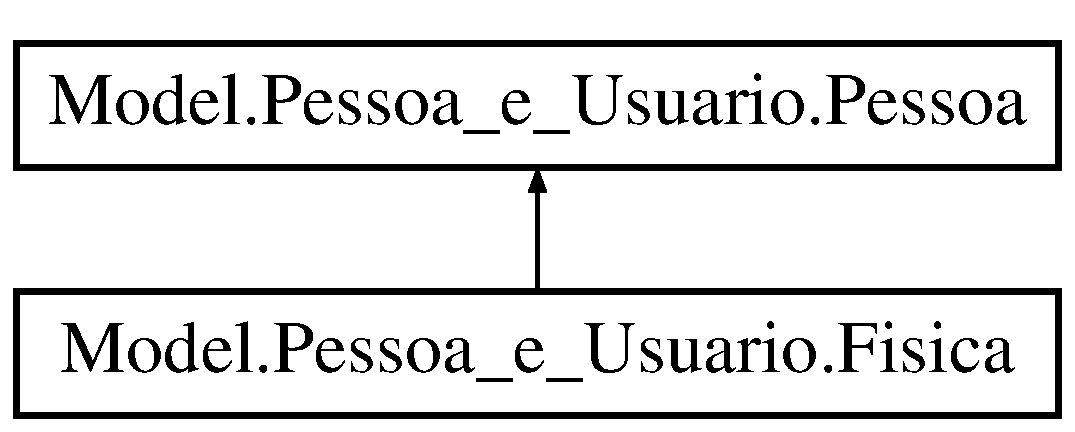
\includegraphics[height=2.000000cm]{class_model_1_1_pessoa__e___usuario_1_1_fisica}
\end{center}
\end{figure}
\subsection*{Membros públicos}
\begin{DoxyCompactItemize}
\item 
String \hyperlink{class_model_1_1_pessoa__e___usuario_1_1_fisica_a6938671249e215e455665ce5084b5c9b}{Save} (String \+\_\+nome, String \+\_\+endereco, string \+\_\+telefone, string \+\_\+situacao, string \+\_\+sigla\+Estado, string \+\_\+cidade, string \+\_\+bairro, string \+\_\+cep, string \+\_\+observacoes, string \+\_\+cpf, string \+\_\+celular, string \+\_\+sexo, Date\+Time \+\_\+datadenascimento)
\begin{DoxyCompactList}\small\item\em Salvando pessoa Física na pasta \char`\"{}\+F\char`\"{}(Pasta usada para guardar todas as pessoas físicas no diretorio do software). \end{DoxyCompactList}\item 
\hyperlink{class_model_1_1_pessoa__e___usuario_1_1_fisica}{Fisica} \hyperlink{class_model_1_1_pessoa__e___usuario_1_1_fisica_a13ff6dd977b906babecb398560d8601e}{Load} (String \+\_\+\+Nome)
\begin{DoxyCompactList}\small\item\em Carregando pessoa Física. \end{DoxyCompactList}\item 
List$<$ string $>$ \hyperlink{class_model_1_1_pessoa__e___usuario_1_1_fisica_a9f771ef7f7b741221c0821a1a0547318}{Load\+List} ()
\begin{DoxyCompactList}\small\item\em Carregando Lista com nome de todas pessoas Físicas registradas. \end{DoxyCompactList}\item 
bool \hyperlink{class_model_1_1_pessoa__e___usuario_1_1_fisica_a2084087f39edc38a532ebbc07811202d}{Verificar} (String \+\_\+nome)
\begin{DoxyCompactList}\small\item\em Verificando de a \char`\"{}\+Pessoa física\char`\"{} existe. \end{DoxyCompactList}\end{DoxyCompactItemize}
\subsection*{Propriedades}
\begin{DoxyCompactItemize}
\item 
\hypertarget{class_model_1_1_pessoa__e___usuario_1_1_fisica_a29515077dfb355670b8c0a7d7ebe994b}{}string {\bfseries Sexo}\hspace{0.3cm}{\ttfamily  \mbox{[}get, set\mbox{]}}\label{class_model_1_1_pessoa__e___usuario_1_1_fisica_a29515077dfb355670b8c0a7d7ebe994b}

\item 
\hypertarget{class_model_1_1_pessoa__e___usuario_1_1_fisica_a2baa5ada8c7dd8be142e08abd58b21c3}{}string {\bfseries C\+P\+F}\hspace{0.3cm}{\ttfamily  \mbox{[}get, set\mbox{]}}\label{class_model_1_1_pessoa__e___usuario_1_1_fisica_a2baa5ada8c7dd8be142e08abd58b21c3}

\item 
\hypertarget{class_model_1_1_pessoa__e___usuario_1_1_fisica_ac87cd88aaa7c64a5208f9aa25b4f7cf8}{}string {\bfseries Celular}\hspace{0.3cm}{\ttfamily  \mbox{[}get, set\mbox{]}}\label{class_model_1_1_pessoa__e___usuario_1_1_fisica_ac87cd88aaa7c64a5208f9aa25b4f7cf8}

\item 
\hypertarget{class_model_1_1_pessoa__e___usuario_1_1_fisica_afa181c961f544f9da0e9bd76a6f7dc1b}{}Date\+Time {\bfseries Data\+De\+Nascimento}\hspace{0.3cm}{\ttfamily  \mbox{[}get, set\mbox{]}}\label{class_model_1_1_pessoa__e___usuario_1_1_fisica_afa181c961f544f9da0e9bd76a6f7dc1b}

\end{DoxyCompactItemize}


\subsection{Documentação dos métodos}
\hypertarget{class_model_1_1_pessoa__e___usuario_1_1_fisica_a13ff6dd977b906babecb398560d8601e}{}\index{Model\+::\+Pessoa\+\_\+e\+\_\+\+Usuario\+::\+Fisica@{Model\+::\+Pessoa\+\_\+e\+\_\+\+Usuario\+::\+Fisica}!Load@{Load}}
\index{Load@{Load}!Model\+::\+Pessoa\+\_\+e\+\_\+\+Usuario\+::\+Fisica@{Model\+::\+Pessoa\+\_\+e\+\_\+\+Usuario\+::\+Fisica}}
\subsubsection[{Load(\+String \+\_\+\+Nome)}]{\setlength{\rightskip}{0pt plus 5cm}{\bf Fisica} Model.\+Pessoa\+\_\+e\+\_\+\+Usuario.\+Fisica.\+Load (
\begin{DoxyParamCaption}
\item[{String}]{\+\_\+\+Nome}
\end{DoxyParamCaption}
)}\label{class_model_1_1_pessoa__e___usuario_1_1_fisica_a13ff6dd977b906babecb398560d8601e}


Carregando pessoa Física. 


\begin{DoxyParams}{Parâmetros}
{\em \+\_\+\+Nome} & \\
\hline
\end{DoxyParams}
\begin{DoxyReturn}{Retorna}
\hyperlink{class_model_1_1_pessoa__e___usuario_1_1_pessoa}{Pessoa} Física
\end{DoxyReturn}
\hypertarget{class_model_1_1_pessoa__e___usuario_1_1_fisica_a9f771ef7f7b741221c0821a1a0547318}{}\index{Model\+::\+Pessoa\+\_\+e\+\_\+\+Usuario\+::\+Fisica@{Model\+::\+Pessoa\+\_\+e\+\_\+\+Usuario\+::\+Fisica}!Load\+List@{Load\+List}}
\index{Load\+List@{Load\+List}!Model\+::\+Pessoa\+\_\+e\+\_\+\+Usuario\+::\+Fisica@{Model\+::\+Pessoa\+\_\+e\+\_\+\+Usuario\+::\+Fisica}}
\subsubsection[{Load\+List()}]{\setlength{\rightskip}{0pt plus 5cm}List$<$string$>$ Model.\+Pessoa\+\_\+e\+\_\+\+Usuario.\+Fisica.\+Load\+List (
\begin{DoxyParamCaption}
{}
\end{DoxyParamCaption}
)}\label{class_model_1_1_pessoa__e___usuario_1_1_fisica_a9f771ef7f7b741221c0821a1a0547318}


Carregando Lista com nome de todas pessoas Físicas registradas. 

\begin{DoxyReturn}{Retorna}
Lista de nomes.
\end{DoxyReturn}
\hypertarget{class_model_1_1_pessoa__e___usuario_1_1_fisica_a6938671249e215e455665ce5084b5c9b}{}\index{Model\+::\+Pessoa\+\_\+e\+\_\+\+Usuario\+::\+Fisica@{Model\+::\+Pessoa\+\_\+e\+\_\+\+Usuario\+::\+Fisica}!Save@{Save}}
\index{Save@{Save}!Model\+::\+Pessoa\+\_\+e\+\_\+\+Usuario\+::\+Fisica@{Model\+::\+Pessoa\+\_\+e\+\_\+\+Usuario\+::\+Fisica}}
\subsubsection[{Save(\+String \+\_\+nome, String \+\_\+endereco, string \+\_\+telefone, string \+\_\+situacao, string \+\_\+sigla\+Estado, string \+\_\+cidade, string \+\_\+bairro, string \+\_\+cep, string \+\_\+observacoes, string \+\_\+cpf, string \+\_\+celular, string \+\_\+sexo, Date\+Time \+\_\+datadenascimento)}]{\setlength{\rightskip}{0pt plus 5cm}String Model.\+Pessoa\+\_\+e\+\_\+\+Usuario.\+Fisica.\+Save (
\begin{DoxyParamCaption}
\item[{String}]{\+\_\+nome, }
\item[{String}]{\+\_\+endereco, }
\item[{string}]{\+\_\+telefone, }
\item[{string}]{\+\_\+situacao, }
\item[{string}]{\+\_\+sigla\+Estado, }
\item[{string}]{\+\_\+cidade, }
\item[{string}]{\+\_\+bairro, }
\item[{string}]{\+\_\+cep, }
\item[{string}]{\+\_\+observacoes, }
\item[{string}]{\+\_\+cpf, }
\item[{string}]{\+\_\+celular, }
\item[{string}]{\+\_\+sexo, }
\item[{Date\+Time}]{\+\_\+datadenascimento}
\end{DoxyParamCaption}
)}\label{class_model_1_1_pessoa__e___usuario_1_1_fisica_a6938671249e215e455665ce5084b5c9b}


Salvando pessoa Física na pasta \char`\"{}\+F\char`\"{}(Pasta usada para guardar todas as pessoas físicas no diretorio do software). 


\begin{DoxyParams}{Parâmetros}
{\em \+\_\+nome} & \\
\hline
{\em \+\_\+endereco} & \\
\hline
{\em \+\_\+telefone} & \\
\hline
{\em \+\_\+situacao} & \\
\hline
{\em \+\_\+sigla\+Estado} & \\
\hline
{\em \+\_\+cidade} & \\
\hline
{\em \+\_\+bairro} & \\
\hline
{\em \+\_\+cep} & \\
\hline
{\em \+\_\+observacoes} & \\
\hline
{\em \+\_\+cpf} & \\
\hline
{\em \+\_\+celular} & \\
\hline
{\em \+\_\+sexo} & \\
\hline
{\em \+\_\+datadenascimento} & \\
\hline
\end{DoxyParams}
\begin{DoxyReturn}{Retorna}

\end{DoxyReturn}
\hypertarget{class_model_1_1_pessoa__e___usuario_1_1_fisica_a2084087f39edc38a532ebbc07811202d}{}\index{Model\+::\+Pessoa\+\_\+e\+\_\+\+Usuario\+::\+Fisica@{Model\+::\+Pessoa\+\_\+e\+\_\+\+Usuario\+::\+Fisica}!Verificar@{Verificar}}
\index{Verificar@{Verificar}!Model\+::\+Pessoa\+\_\+e\+\_\+\+Usuario\+::\+Fisica@{Model\+::\+Pessoa\+\_\+e\+\_\+\+Usuario\+::\+Fisica}}
\subsubsection[{Verificar(\+String \+\_\+nome)}]{\setlength{\rightskip}{0pt plus 5cm}bool Model.\+Pessoa\+\_\+e\+\_\+\+Usuario.\+Fisica.\+Verificar (
\begin{DoxyParamCaption}
\item[{String}]{\+\_\+nome}
\end{DoxyParamCaption}
)}\label{class_model_1_1_pessoa__e___usuario_1_1_fisica_a2084087f39edc38a532ebbc07811202d}


Verificando de a \char`\"{}\+Pessoa física\char`\"{} existe. 


\begin{DoxyParams}{Parâmetros}
{\em \+\_\+nome} & \\
\hline
\end{DoxyParams}
\begin{DoxyReturn}{Retorna}

\end{DoxyReturn}


A documentação para esta classe foi gerada a partir do seguinte ficheiro\+:\begin{DoxyCompactItemize}
\item 
D\+:/\+Projetos/\+Software\+Ordem\+De\+Servico/\+Model/\+Pessoa e Usuario/Fisica.\+cs\end{DoxyCompactItemize}

\hypertarget{class_view_1_1_frm___backup}{}\section{Referência à classe View.\+Frm\+\_\+\+Backup}
\label{class_view_1_1_frm___backup}\index{View.\+Frm\+\_\+\+Backup@{View.\+Frm\+\_\+\+Backup}}
Diagrama de heranças da classe View.\+Frm\+\_\+\+Backup\begin{figure}[H]
\begin{center}
\leavevmode
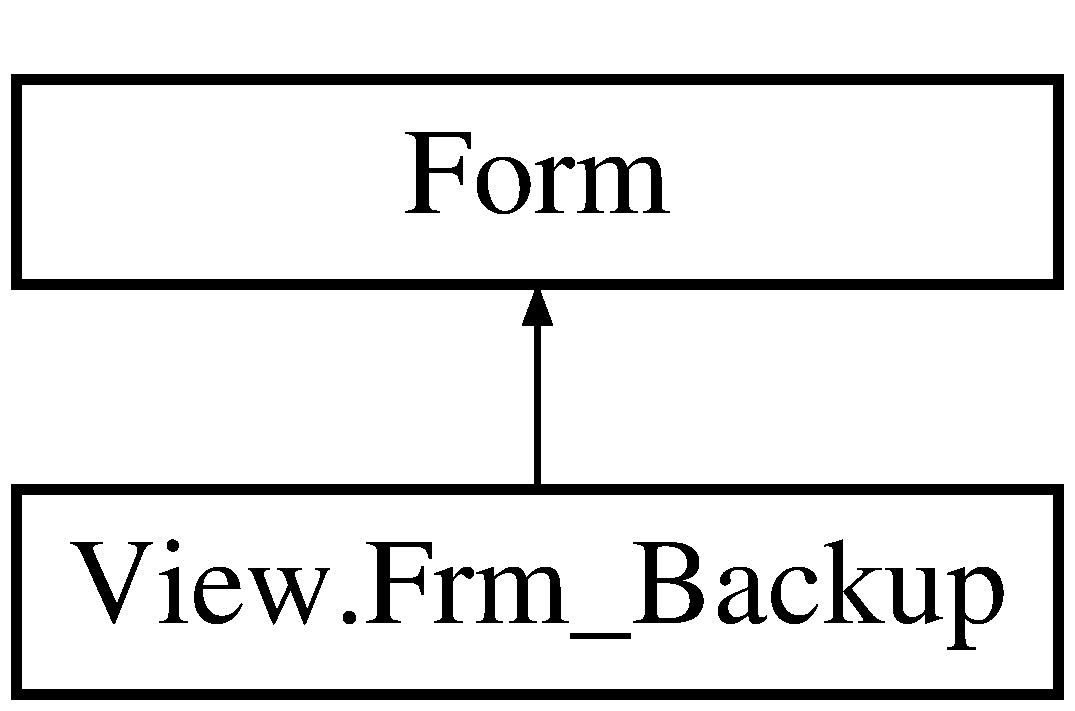
\includegraphics[height=2.000000cm]{class_view_1_1_frm___backup}
\end{center}
\end{figure}
\subsection*{Membros protegidos}
\begin{DoxyCompactItemize}
\item 
override void \hyperlink{class_view_1_1_frm___backup_a0ed544e5c7234a7399ddaa64f8a11c97}{Dispose} (bool disposing)
\begin{DoxyCompactList}\small\item\em Clean up any resources being used. \end{DoxyCompactList}\end{DoxyCompactItemize}


\subsection{Documentação dos métodos}
\hypertarget{class_view_1_1_frm___backup_a0ed544e5c7234a7399ddaa64f8a11c97}{}\index{View\+::\+Frm\+\_\+\+Backup@{View\+::\+Frm\+\_\+\+Backup}!Dispose@{Dispose}}
\index{Dispose@{Dispose}!View\+::\+Frm\+\_\+\+Backup@{View\+::\+Frm\+\_\+\+Backup}}
\subsubsection[{Dispose(bool disposing)}]{\setlength{\rightskip}{0pt plus 5cm}override void View.\+Frm\+\_\+\+Backup.\+Dispose (
\begin{DoxyParamCaption}
\item[{bool}]{disposing}
\end{DoxyParamCaption}
)\hspace{0.3cm}{\ttfamily [protected]}}\label{class_view_1_1_frm___backup_a0ed544e5c7234a7399ddaa64f8a11c97}


Clean up any resources being used. 


\begin{DoxyParams}{Parâmetros}
{\em disposing} & true if managed resources should be disposed; otherwise, false.\\
\hline
\end{DoxyParams}


A documentação para esta classe foi gerada a partir dos seguintes ficheiros\+:\begin{DoxyCompactItemize}
\item 
D\+:/\+Projetos/\+Software\+Ordem\+De\+Servico/\+View/\+Outros/Frm\+\_\+\+Backup.\+cs\item 
D\+:/\+Projetos/\+Software\+Ordem\+De\+Servico/\+View/\+Outros/Frm\+\_\+\+Backup.\+Designer.\+cs\end{DoxyCompactItemize}

\hypertarget{class_view_1_1_o_s_1_1_frm___editar_o_s}{}\section{Referência à classe View.\+O\+S.\+Frm\+\_\+\+Editar\+O\+S}
\label{class_view_1_1_o_s_1_1_frm___editar_o_s}\index{View.\+O\+S.\+Frm\+\_\+\+Editar\+O\+S@{View.\+O\+S.\+Frm\+\_\+\+Editar\+O\+S}}
Diagrama de heranças da classe View.\+O\+S.\+Frm\+\_\+\+Editar\+O\+S\begin{figure}[H]
\begin{center}
\leavevmode
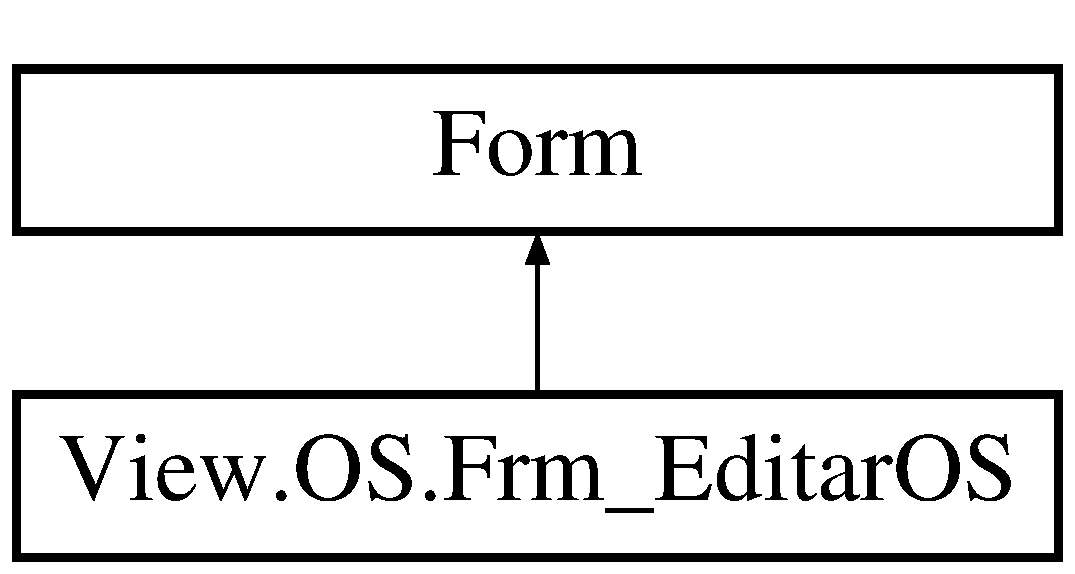
\includegraphics[height=2.000000cm]{class_view_1_1_o_s_1_1_frm___editar_o_s}
\end{center}
\end{figure}
\subsection*{Membros protegidos}
\begin{DoxyCompactItemize}
\item 
override void \hyperlink{class_view_1_1_o_s_1_1_frm___editar_o_s_a51231aa310acaa75ee0d8d4bb31b2291}{Dispose} (bool disposing)
\begin{DoxyCompactList}\small\item\em Clean up any resources being used. \end{DoxyCompactList}\end{DoxyCompactItemize}


\subsection{Documentação dos métodos}
\hypertarget{class_view_1_1_o_s_1_1_frm___editar_o_s_a51231aa310acaa75ee0d8d4bb31b2291}{}\index{View\+::\+O\+S\+::\+Frm\+\_\+\+Editar\+O\+S@{View\+::\+O\+S\+::\+Frm\+\_\+\+Editar\+O\+S}!Dispose@{Dispose}}
\index{Dispose@{Dispose}!View\+::\+O\+S\+::\+Frm\+\_\+\+Editar\+O\+S@{View\+::\+O\+S\+::\+Frm\+\_\+\+Editar\+O\+S}}
\subsubsection[{Dispose(bool disposing)}]{\setlength{\rightskip}{0pt plus 5cm}override void View.\+O\+S.\+Frm\+\_\+\+Editar\+O\+S.\+Dispose (
\begin{DoxyParamCaption}
\item[{bool}]{disposing}
\end{DoxyParamCaption}
)\hspace{0.3cm}{\ttfamily [protected]}}\label{class_view_1_1_o_s_1_1_frm___editar_o_s_a51231aa310acaa75ee0d8d4bb31b2291}


Clean up any resources being used. 


\begin{DoxyParams}{Parâmetros}
{\em disposing} & true if managed resources should be disposed; otherwise, false.\\
\hline
\end{DoxyParams}


A documentação para esta classe foi gerada a partir dos seguintes ficheiros\+:\begin{DoxyCompactItemize}
\item 
C\+:/\+Cristiano/\+Projetos/\+Software\+Ordem\+De\+Servico/\+View/\+O\+S/Frm\+\_\+\+Editar\+O\+S.\+cs\item 
C\+:/\+Cristiano/\+Projetos/\+Software\+Ordem\+De\+Servico/\+View/\+O\+S/Frm\+\_\+\+Editar\+O\+S.\+Designer.\+cs\end{DoxyCompactItemize}

\hypertarget{class_view_1_1_usuario_1_1_frm___edit_usu}{}\section{Referência à classe View.\+Usuario.\+Frm\+\_\+\+Edit\+Usu}
\label{class_view_1_1_usuario_1_1_frm___edit_usu}\index{View.\+Usuario.\+Frm\+\_\+\+Edit\+Usu@{View.\+Usuario.\+Frm\+\_\+\+Edit\+Usu}}
Diagrama de heranças da classe View.\+Usuario.\+Frm\+\_\+\+Edit\+Usu\begin{figure}[H]
\begin{center}
\leavevmode
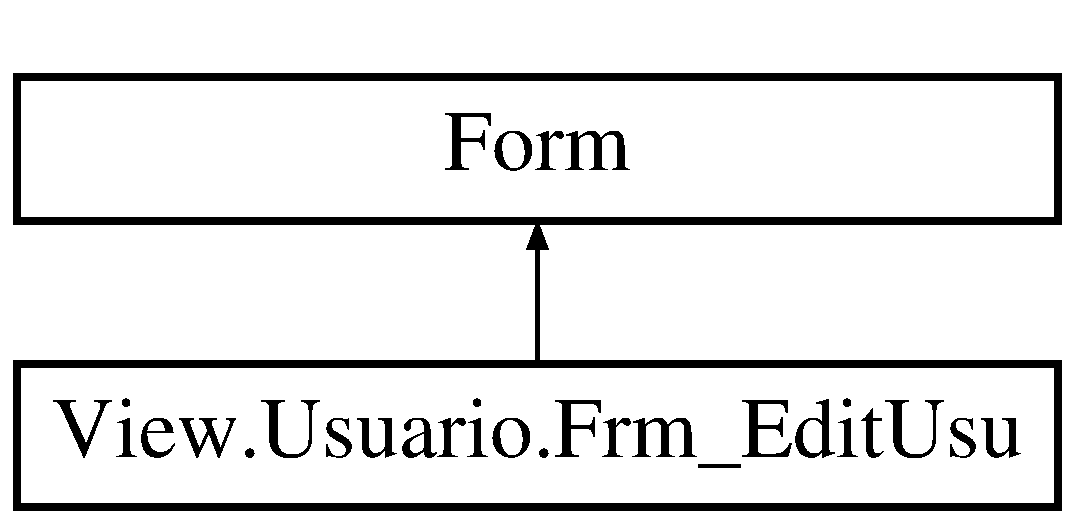
\includegraphics[height=2.000000cm]{class_view_1_1_usuario_1_1_frm___edit_usu}
\end{center}
\end{figure}
\subsection*{Membros protegidos}
\begin{DoxyCompactItemize}
\item 
override void \hyperlink{class_view_1_1_usuario_1_1_frm___edit_usu_abe35c56b13abb84f233aa0fd27635dac}{Dispose} (bool disposing)
\begin{DoxyCompactList}\small\item\em Clean up any resources being used. \end{DoxyCompactList}\end{DoxyCompactItemize}


\subsection{Documentação dos métodos}
\hypertarget{class_view_1_1_usuario_1_1_frm___edit_usu_abe35c56b13abb84f233aa0fd27635dac}{}\index{View\+::\+Usuario\+::\+Frm\+\_\+\+Edit\+Usu@{View\+::\+Usuario\+::\+Frm\+\_\+\+Edit\+Usu}!Dispose@{Dispose}}
\index{Dispose@{Dispose}!View\+::\+Usuario\+::\+Frm\+\_\+\+Edit\+Usu@{View\+::\+Usuario\+::\+Frm\+\_\+\+Edit\+Usu}}
\subsubsection[{Dispose(bool disposing)}]{\setlength{\rightskip}{0pt plus 5cm}override void View.\+Usuario.\+Frm\+\_\+\+Edit\+Usu.\+Dispose (
\begin{DoxyParamCaption}
\item[{bool}]{disposing}
\end{DoxyParamCaption}
)\hspace{0.3cm}{\ttfamily [protected]}}\label{class_view_1_1_usuario_1_1_frm___edit_usu_abe35c56b13abb84f233aa0fd27635dac}


Clean up any resources being used. 


\begin{DoxyParams}{Parâmetros}
{\em disposing} & true if managed resources should be disposed; otherwise, false.\\
\hline
\end{DoxyParams}


A documentação para esta classe foi gerada a partir dos seguintes ficheiros\+:\begin{DoxyCompactItemize}
\item 
C\+:/\+Cristiano/\+Projetos/\+Software\+Ordem\+De\+Servico/\+View/\+Usuario/Frm\+\_\+\+Edit\+Usu.\+cs\item 
C\+:/\+Cristiano/\+Projetos/\+Software\+Ordem\+De\+Servico/\+View/\+Usuario/Frm\+\_\+\+Edit\+Usu.\+Designer.\+cs\end{DoxyCompactItemize}

\hypertarget{class_view_1_1_frm___imprimir_o_s}{}\section{Referência à classe View.\+Frm\+\_\+\+Imprimir\+O\+S}
\label{class_view_1_1_frm___imprimir_o_s}\index{View.\+Frm\+\_\+\+Imprimir\+O\+S@{View.\+Frm\+\_\+\+Imprimir\+O\+S}}
Diagrama de heranças da classe View.\+Frm\+\_\+\+Imprimir\+O\+S\begin{figure}[H]
\begin{center}
\leavevmode
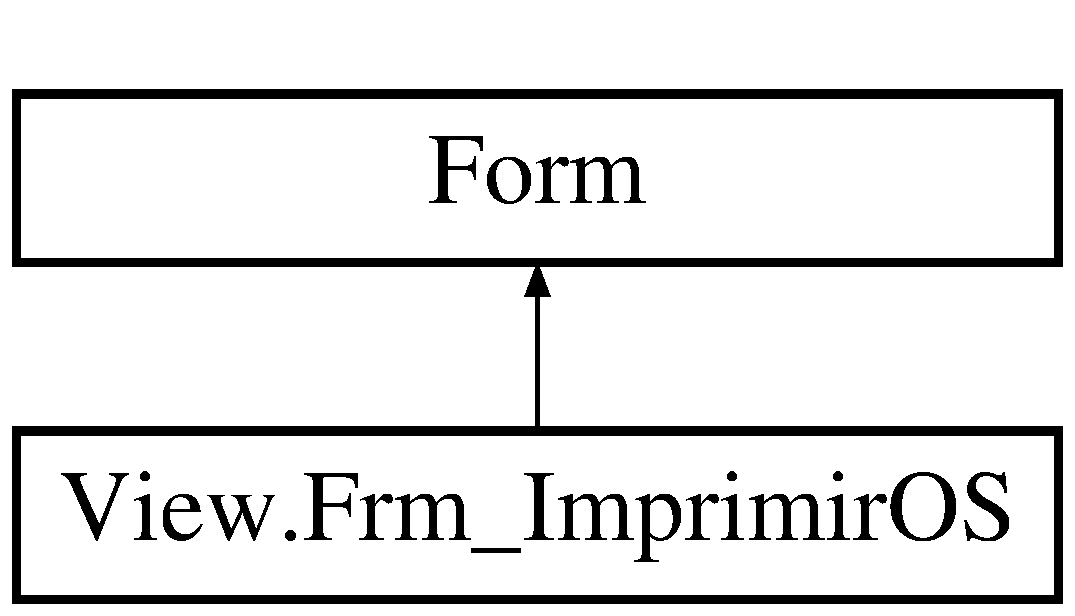
\includegraphics[height=2.000000cm]{class_view_1_1_frm___imprimir_o_s}
\end{center}
\end{figure}
\subsection*{Membros protegidos}
\begin{DoxyCompactItemize}
\item 
override void \hyperlink{class_view_1_1_frm___imprimir_o_s_aa9822f5e5d38db035f2f89b3e06bf07d}{Dispose} (bool disposing)
\begin{DoxyCompactList}\small\item\em Clean up any resources being used. \end{DoxyCompactList}\end{DoxyCompactItemize}


\subsection{Documentação dos métodos}
\hypertarget{class_view_1_1_frm___imprimir_o_s_aa9822f5e5d38db035f2f89b3e06bf07d}{}\index{View\+::\+Frm\+\_\+\+Imprimir\+O\+S@{View\+::\+Frm\+\_\+\+Imprimir\+O\+S}!Dispose@{Dispose}}
\index{Dispose@{Dispose}!View\+::\+Frm\+\_\+\+Imprimir\+O\+S@{View\+::\+Frm\+\_\+\+Imprimir\+O\+S}}
\subsubsection[{Dispose(bool disposing)}]{\setlength{\rightskip}{0pt plus 5cm}override void View.\+Frm\+\_\+\+Imprimir\+O\+S.\+Dispose (
\begin{DoxyParamCaption}
\item[{bool}]{disposing}
\end{DoxyParamCaption}
)\hspace{0.3cm}{\ttfamily [protected]}}\label{class_view_1_1_frm___imprimir_o_s_aa9822f5e5d38db035f2f89b3e06bf07d}


Clean up any resources being used. 


\begin{DoxyParams}{Parâmetros}
{\em disposing} & true if managed resources should be disposed; otherwise, false.\\
\hline
\end{DoxyParams}


A documentação para esta classe foi gerada a partir dos seguintes ficheiros\+:\begin{DoxyCompactItemize}
\item 
D\+:/\+Projetos/\+Software\+Ordem\+De\+Servico/\+View/\+O\+S/Frm\+\_\+\+Imprimir\+O\+S.\+cs\item 
D\+:/\+Projetos/\+Software\+Ordem\+De\+Servico/\+View/\+O\+S/Frm\+\_\+\+Imprimir\+O\+S.\+Designer.\+cs\end{DoxyCompactItemize}

\hypertarget{class_view_1_1_pessoas_1_1_frm___listar_fisica}{}\section{Referência à classe View.\+Pessoas.\+Frm\+\_\+\+Listar\+Fisica}
\label{class_view_1_1_pessoas_1_1_frm___listar_fisica}\index{View.\+Pessoas.\+Frm\+\_\+\+Listar\+Fisica@{View.\+Pessoas.\+Frm\+\_\+\+Listar\+Fisica}}
Diagrama de heranças da classe View.\+Pessoas.\+Frm\+\_\+\+Listar\+Fisica\begin{figure}[H]
\begin{center}
\leavevmode
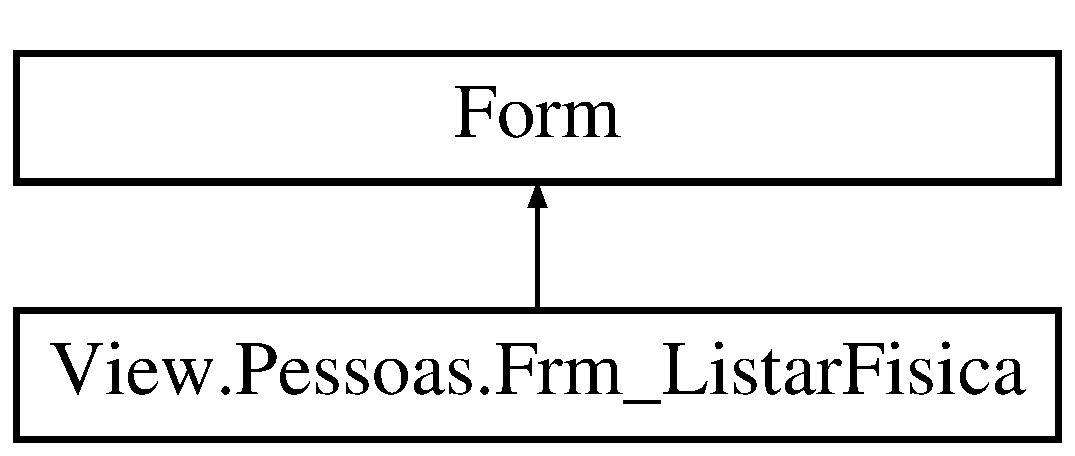
\includegraphics[height=2.000000cm]{class_view_1_1_pessoas_1_1_frm___listar_fisica}
\end{center}
\end{figure}
\subsection*{Membros protegidos}
\begin{DoxyCompactItemize}
\item 
override void \hyperlink{class_view_1_1_pessoas_1_1_frm___listar_fisica_a50eb1e2c5bd7b1e123a76c0e67257833}{Dispose} (bool disposing)
\begin{DoxyCompactList}\small\item\em Clean up any resources being used. \end{DoxyCompactList}\end{DoxyCompactItemize}


\subsection{Documentação dos métodos}
\hypertarget{class_view_1_1_pessoas_1_1_frm___listar_fisica_a50eb1e2c5bd7b1e123a76c0e67257833}{}\index{View\+::\+Pessoas\+::\+Frm\+\_\+\+Listar\+Fisica@{View\+::\+Pessoas\+::\+Frm\+\_\+\+Listar\+Fisica}!Dispose@{Dispose}}
\index{Dispose@{Dispose}!View\+::\+Pessoas\+::\+Frm\+\_\+\+Listar\+Fisica@{View\+::\+Pessoas\+::\+Frm\+\_\+\+Listar\+Fisica}}
\subsubsection[{Dispose(bool disposing)}]{\setlength{\rightskip}{0pt plus 5cm}override void View.\+Pessoas.\+Frm\+\_\+\+Listar\+Fisica.\+Dispose (
\begin{DoxyParamCaption}
\item[{bool}]{disposing}
\end{DoxyParamCaption}
)\hspace{0.3cm}{\ttfamily [protected]}}\label{class_view_1_1_pessoas_1_1_frm___listar_fisica_a50eb1e2c5bd7b1e123a76c0e67257833}


Clean up any resources being used. 


\begin{DoxyParams}{Parâmetros}
{\em disposing} & true if managed resources should be disposed; otherwise, false.\\
\hline
\end{DoxyParams}


A documentação para esta classe foi gerada a partir dos seguintes ficheiros\+:\begin{DoxyCompactItemize}
\item 
C\+:/\+Cristiano/\+Projetos/\+Software\+Ordem\+De\+Servico/\+View/\+Pessoas/Frm\+\_\+\+Listar\+Fisica.\+cs\item 
C\+:/\+Cristiano/\+Projetos/\+Software\+Ordem\+De\+Servico/\+View/\+Pessoas/Frm\+\_\+\+Listar\+Fisica.\+Designer.\+cs\end{DoxyCompactItemize}

\hypertarget{class_view_1_1_pessoas_1_1_frm___listar_juridica}{}\section{Referência à classe View.\+Pessoas.\+Frm\+\_\+\+Listar\+Juridica}
\label{class_view_1_1_pessoas_1_1_frm___listar_juridica}\index{View.\+Pessoas.\+Frm\+\_\+\+Listar\+Juridica@{View.\+Pessoas.\+Frm\+\_\+\+Listar\+Juridica}}
Diagrama de heranças da classe View.\+Pessoas.\+Frm\+\_\+\+Listar\+Juridica\begin{figure}[H]
\begin{center}
\leavevmode
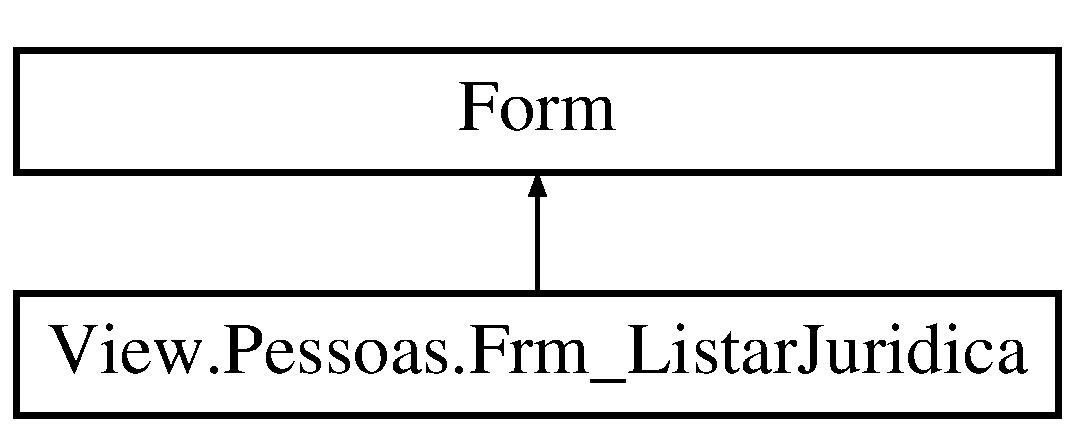
\includegraphics[height=2.000000cm]{class_view_1_1_pessoas_1_1_frm___listar_juridica}
\end{center}
\end{figure}
\subsection*{Membros protegidos}
\begin{DoxyCompactItemize}
\item 
override void \hyperlink{class_view_1_1_pessoas_1_1_frm___listar_juridica_a774819568069390493fffb4ef69d306c}{Dispose} (bool disposing)
\begin{DoxyCompactList}\small\item\em Clean up any resources being used. \end{DoxyCompactList}\end{DoxyCompactItemize}


\subsection{Documentação dos métodos}
\hypertarget{class_view_1_1_pessoas_1_1_frm___listar_juridica_a774819568069390493fffb4ef69d306c}{}\index{View\+::\+Pessoas\+::\+Frm\+\_\+\+Listar\+Juridica@{View\+::\+Pessoas\+::\+Frm\+\_\+\+Listar\+Juridica}!Dispose@{Dispose}}
\index{Dispose@{Dispose}!View\+::\+Pessoas\+::\+Frm\+\_\+\+Listar\+Juridica@{View\+::\+Pessoas\+::\+Frm\+\_\+\+Listar\+Juridica}}
\subsubsection[{Dispose(bool disposing)}]{\setlength{\rightskip}{0pt plus 5cm}override void View.\+Pessoas.\+Frm\+\_\+\+Listar\+Juridica.\+Dispose (
\begin{DoxyParamCaption}
\item[{bool}]{disposing}
\end{DoxyParamCaption}
)\hspace{0.3cm}{\ttfamily [protected]}}\label{class_view_1_1_pessoas_1_1_frm___listar_juridica_a774819568069390493fffb4ef69d306c}


Clean up any resources being used. 


\begin{DoxyParams}{Parâmetros}
{\em disposing} & true if managed resources should be disposed; otherwise, false.\\
\hline
\end{DoxyParams}


A documentação para esta classe foi gerada a partir dos seguintes ficheiros\+:\begin{DoxyCompactItemize}
\item 
D\+:/\+Projetos/\+Software\+Ordem\+De\+Servico/\+View/\+Pessoas/Frm\+\_\+\+Listar\+Juridica.\+cs\item 
D\+:/\+Projetos/\+Software\+Ordem\+De\+Servico/\+View/\+Pessoas/Frm\+\_\+\+Listar\+Juridica.\+Designer.\+cs\end{DoxyCompactItemize}

\hypertarget{class_view_1_1_o_s_1_1_frm___listar_o_s}{}\section{Referência à classe View.\+O\+S.\+Frm\+\_\+\+Listar\+O\+S}
\label{class_view_1_1_o_s_1_1_frm___listar_o_s}\index{View.\+O\+S.\+Frm\+\_\+\+Listar\+O\+S@{View.\+O\+S.\+Frm\+\_\+\+Listar\+O\+S}}
Diagrama de heranças da classe View.\+O\+S.\+Frm\+\_\+\+Listar\+O\+S\begin{figure}[H]
\begin{center}
\leavevmode
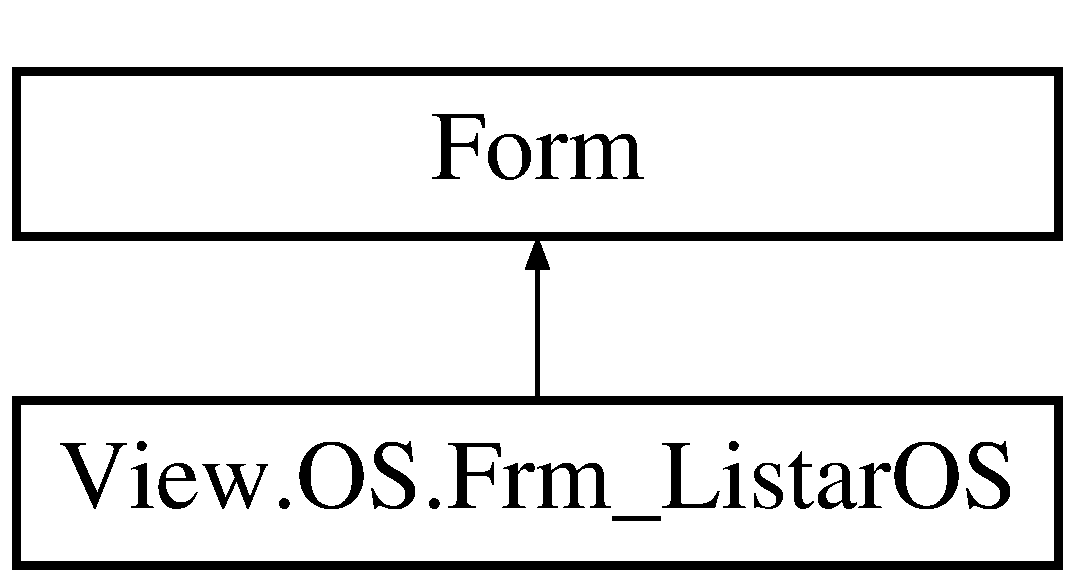
\includegraphics[height=2.000000cm]{class_view_1_1_o_s_1_1_frm___listar_o_s}
\end{center}
\end{figure}
\subsection*{Membros protegidos}
\begin{DoxyCompactItemize}
\item 
override void \hyperlink{class_view_1_1_o_s_1_1_frm___listar_o_s_a912a6dd9c258cfd7312572e0ef17c23e}{Dispose} (bool disposing)
\begin{DoxyCompactList}\small\item\em Clean up any resources being used. \end{DoxyCompactList}\end{DoxyCompactItemize}


\subsection{Documentação dos métodos}
\hypertarget{class_view_1_1_o_s_1_1_frm___listar_o_s_a912a6dd9c258cfd7312572e0ef17c23e}{}\index{View\+::\+O\+S\+::\+Frm\+\_\+\+Listar\+O\+S@{View\+::\+O\+S\+::\+Frm\+\_\+\+Listar\+O\+S}!Dispose@{Dispose}}
\index{Dispose@{Dispose}!View\+::\+O\+S\+::\+Frm\+\_\+\+Listar\+O\+S@{View\+::\+O\+S\+::\+Frm\+\_\+\+Listar\+O\+S}}
\subsubsection[{Dispose(bool disposing)}]{\setlength{\rightskip}{0pt plus 5cm}override void View.\+O\+S.\+Frm\+\_\+\+Listar\+O\+S.\+Dispose (
\begin{DoxyParamCaption}
\item[{bool}]{disposing}
\end{DoxyParamCaption}
)\hspace{0.3cm}{\ttfamily [protected]}}\label{class_view_1_1_o_s_1_1_frm___listar_o_s_a912a6dd9c258cfd7312572e0ef17c23e}


Clean up any resources being used. 


\begin{DoxyParams}{Parâmetros}
{\em disposing} & true if managed resources should be disposed; otherwise, false.\\
\hline
\end{DoxyParams}


A documentação para esta classe foi gerada a partir dos seguintes ficheiros\+:\begin{DoxyCompactItemize}
\item 
D\+:/\+Projetos/\+Software\+Ordem\+De\+Servico/\+View/\+O\+S/Frm\+\_\+\+Listar\+O\+S.\+cs\item 
D\+:/\+Projetos/\+Software\+Ordem\+De\+Servico/\+View/\+O\+S/Frm\+\_\+\+Listar\+O\+S.\+Designer.\+cs\end{DoxyCompactItemize}

\hypertarget{class_view_1_1_usuario_1_1_frm___listar_usuarios}{}\section{Referência à classe View.\+Usuario.\+Frm\+\_\+\+Listar\+Usuarios}
\label{class_view_1_1_usuario_1_1_frm___listar_usuarios}\index{View.\+Usuario.\+Frm\+\_\+\+Listar\+Usuarios@{View.\+Usuario.\+Frm\+\_\+\+Listar\+Usuarios}}
Diagrama de heranças da classe View.\+Usuario.\+Frm\+\_\+\+Listar\+Usuarios\begin{figure}[H]
\begin{center}
\leavevmode
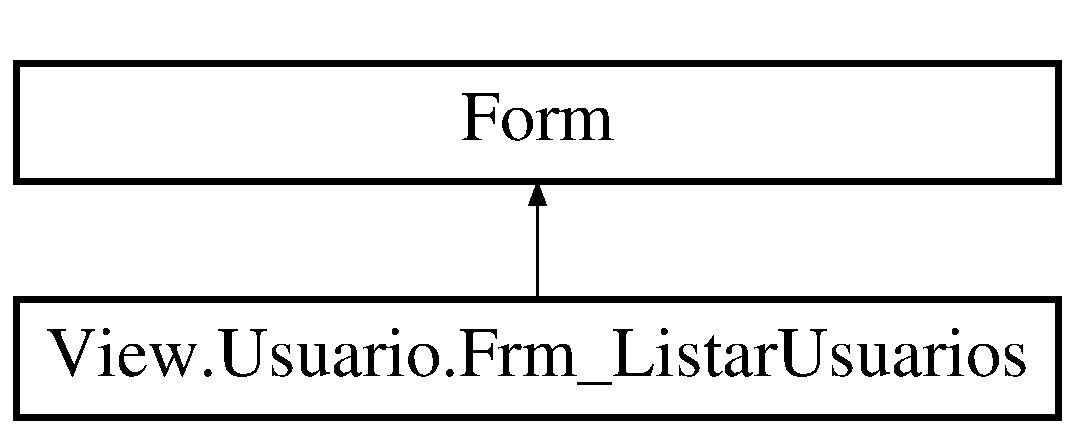
\includegraphics[height=2.000000cm]{class_view_1_1_usuario_1_1_frm___listar_usuarios}
\end{center}
\end{figure}
\subsection*{Membros protegidos}
\begin{DoxyCompactItemize}
\item 
override void \hyperlink{class_view_1_1_usuario_1_1_frm___listar_usuarios_a44ca38b50d8c484cabbe4bb09d211910}{Dispose} (bool disposing)
\begin{DoxyCompactList}\small\item\em Clean up any resources being used. \end{DoxyCompactList}\end{DoxyCompactItemize}


\subsection{Documentação dos métodos}
\hypertarget{class_view_1_1_usuario_1_1_frm___listar_usuarios_a44ca38b50d8c484cabbe4bb09d211910}{}\index{View\+::\+Usuario\+::\+Frm\+\_\+\+Listar\+Usuarios@{View\+::\+Usuario\+::\+Frm\+\_\+\+Listar\+Usuarios}!Dispose@{Dispose}}
\index{Dispose@{Dispose}!View\+::\+Usuario\+::\+Frm\+\_\+\+Listar\+Usuarios@{View\+::\+Usuario\+::\+Frm\+\_\+\+Listar\+Usuarios}}
\subsubsection[{Dispose(bool disposing)}]{\setlength{\rightskip}{0pt plus 5cm}override void View.\+Usuario.\+Frm\+\_\+\+Listar\+Usuarios.\+Dispose (
\begin{DoxyParamCaption}
\item[{bool}]{disposing}
\end{DoxyParamCaption}
)\hspace{0.3cm}{\ttfamily [protected]}}\label{class_view_1_1_usuario_1_1_frm___listar_usuarios_a44ca38b50d8c484cabbe4bb09d211910}


Clean up any resources being used. 


\begin{DoxyParams}{Parâmetros}
{\em disposing} & true if managed resources should be disposed; otherwise, false.\\
\hline
\end{DoxyParams}


A documentação para esta classe foi gerada a partir dos seguintes ficheiros\+:\begin{DoxyCompactItemize}
\item 
C\+:/\+Cristiano/\+Projetos/\+Software\+Ordem\+De\+Servico/\+View/\+Usuario/Frm\+\_\+\+Listar\+Usuarios.\+cs\item 
C\+:/\+Cristiano/\+Projetos/\+Software\+Ordem\+De\+Servico/\+View/\+Usuario/Frm\+\_\+\+Listar\+Usuarios.\+Designer.\+cs\end{DoxyCompactItemize}

\hypertarget{class_view_1_1_frm___login}{}\section{Referência à classe View.\+Frm\+\_\+\+Login}
\label{class_view_1_1_frm___login}\index{View.\+Frm\+\_\+\+Login@{View.\+Frm\+\_\+\+Login}}
Diagrama de heranças da classe View.\+Frm\+\_\+\+Login\begin{figure}[H]
\begin{center}
\leavevmode
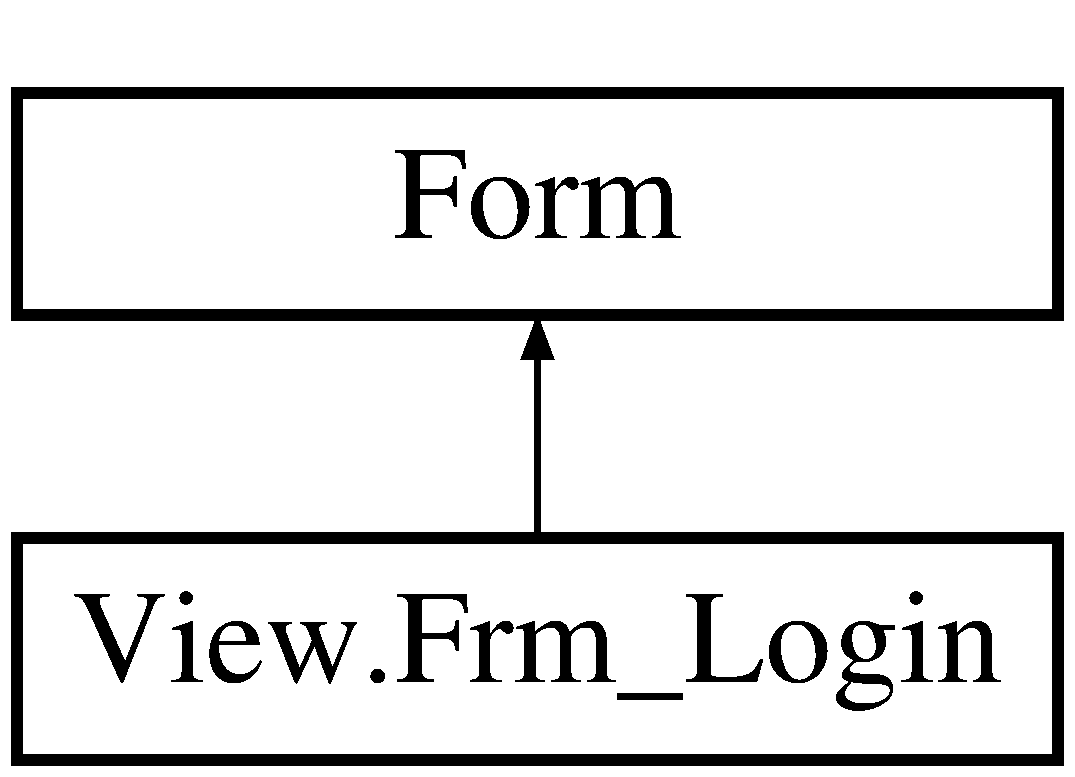
\includegraphics[height=2.000000cm]{class_view_1_1_frm___login}
\end{center}
\end{figure}
\subsection*{Membros protegidos}
\begin{DoxyCompactItemize}
\item 
override void \hyperlink{class_view_1_1_frm___login_a3fe390f393f36fc848cd4b8211ba2be2}{Dispose} (bool disposing)
\begin{DoxyCompactList}\small\item\em Clean up any resources being used. \end{DoxyCompactList}\end{DoxyCompactItemize}


\subsection{Documentação dos métodos}
\hypertarget{class_view_1_1_frm___login_a3fe390f393f36fc848cd4b8211ba2be2}{}\index{View\+::\+Frm\+\_\+\+Login@{View\+::\+Frm\+\_\+\+Login}!Dispose@{Dispose}}
\index{Dispose@{Dispose}!View\+::\+Frm\+\_\+\+Login@{View\+::\+Frm\+\_\+\+Login}}
\subsubsection[{Dispose(bool disposing)}]{\setlength{\rightskip}{0pt plus 5cm}override void View.\+Frm\+\_\+\+Login.\+Dispose (
\begin{DoxyParamCaption}
\item[{bool}]{disposing}
\end{DoxyParamCaption}
)\hspace{0.3cm}{\ttfamily [protected]}}\label{class_view_1_1_frm___login_a3fe390f393f36fc848cd4b8211ba2be2}


Clean up any resources being used. 


\begin{DoxyParams}{Parâmetros}
{\em disposing} & true if managed resources should be disposed; otherwise, false.\\
\hline
\end{DoxyParams}


A documentação para esta classe foi gerada a partir dos seguintes ficheiros\+:\begin{DoxyCompactItemize}
\item 
C\+:/\+Cristiano/\+Projetos/\+Software\+Ordem\+De\+Servico/\+View/\+Outros/Frm\+\_\+\+Login.\+cs\item 
C\+:/\+Cristiano/\+Projetos/\+Software\+Ordem\+De\+Servico/\+View/\+Outros/Frm\+\_\+\+Login.\+Designer.\+cs\end{DoxyCompactItemize}

\hypertarget{class_view_1_1_o_s_1_1_frm___new_ordem}{}\section{Referência à classe View.\+O\+S.\+Frm\+\_\+\+New\+Ordem}
\label{class_view_1_1_o_s_1_1_frm___new_ordem}\index{View.\+O\+S.\+Frm\+\_\+\+New\+Ordem@{View.\+O\+S.\+Frm\+\_\+\+New\+Ordem}}
Diagrama de heranças da classe View.\+O\+S.\+Frm\+\_\+\+New\+Ordem\begin{figure}[H]
\begin{center}
\leavevmode
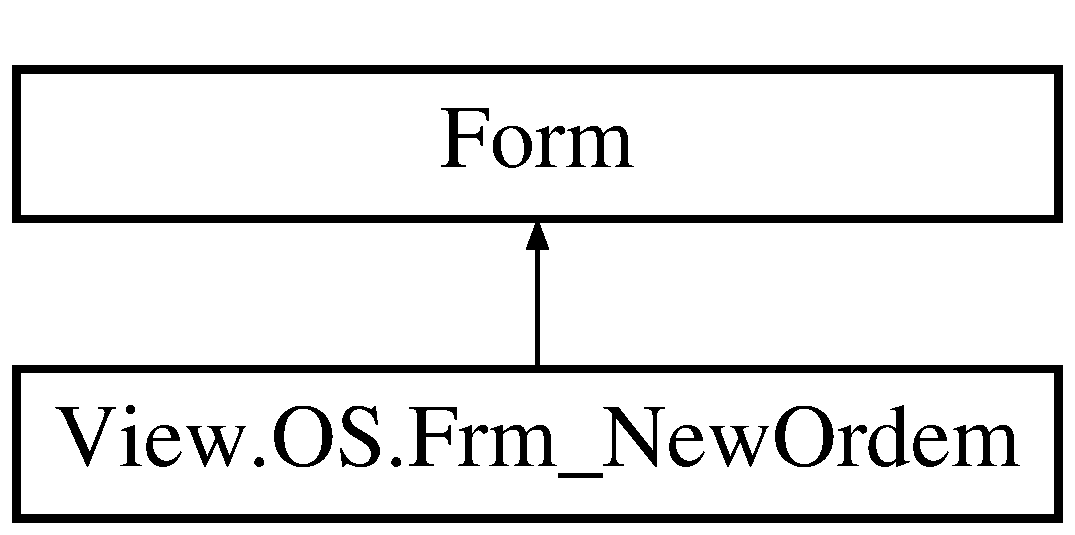
\includegraphics[height=2.000000cm]{class_view_1_1_o_s_1_1_frm___new_ordem}
\end{center}
\end{figure}
\subsection*{Membros protegidos}
\begin{DoxyCompactItemize}
\item 
override void \hyperlink{class_view_1_1_o_s_1_1_frm___new_ordem_a68f1ef63c2a8477814cf81a3a4a3128f}{Dispose} (bool disposing)
\begin{DoxyCompactList}\small\item\em Clean up any resources being used. \end{DoxyCompactList}\end{DoxyCompactItemize}


\subsection{Documentação dos métodos}
\hypertarget{class_view_1_1_o_s_1_1_frm___new_ordem_a68f1ef63c2a8477814cf81a3a4a3128f}{}\index{View\+::\+O\+S\+::\+Frm\+\_\+\+New\+Ordem@{View\+::\+O\+S\+::\+Frm\+\_\+\+New\+Ordem}!Dispose@{Dispose}}
\index{Dispose@{Dispose}!View\+::\+O\+S\+::\+Frm\+\_\+\+New\+Ordem@{View\+::\+O\+S\+::\+Frm\+\_\+\+New\+Ordem}}
\subsubsection[{Dispose(bool disposing)}]{\setlength{\rightskip}{0pt plus 5cm}override void View.\+O\+S.\+Frm\+\_\+\+New\+Ordem.\+Dispose (
\begin{DoxyParamCaption}
\item[{bool}]{disposing}
\end{DoxyParamCaption}
)\hspace{0.3cm}{\ttfamily [protected]}}\label{class_view_1_1_o_s_1_1_frm___new_ordem_a68f1ef63c2a8477814cf81a3a4a3128f}


Clean up any resources being used. 


\begin{DoxyParams}{Parâmetros}
{\em disposing} & true if managed resources should be disposed; otherwise, false.\\
\hline
\end{DoxyParams}


A documentação para esta classe foi gerada a partir dos seguintes ficheiros\+:\begin{DoxyCompactItemize}
\item 
D\+:/\+Projetos/\+Software\+Ordem\+De\+Servico/\+View/\+O\+S/Frm\+\_\+\+New\+Ordem.\+cs\item 
D\+:/\+Projetos/\+Software\+Ordem\+De\+Servico/\+View/\+O\+S/Frm\+\_\+\+New\+Ordem.\+Designer.\+cs\end{DoxyCompactItemize}

\hypertarget{class_view_1_1_formularios___usuarios_1_1_frm___new_usu}{}\section{Referência à classe View.\+Formularios\+\_\+\+Usuarios.\+Frm\+\_\+\+New\+Usu}
\label{class_view_1_1_formularios___usuarios_1_1_frm___new_usu}\index{View.\+Formularios\+\_\+\+Usuarios.\+Frm\+\_\+\+New\+Usu@{View.\+Formularios\+\_\+\+Usuarios.\+Frm\+\_\+\+New\+Usu}}
Diagrama de heranças da classe View.\+Formularios\+\_\+\+Usuarios.\+Frm\+\_\+\+New\+Usu\begin{figure}[H]
\begin{center}
\leavevmode
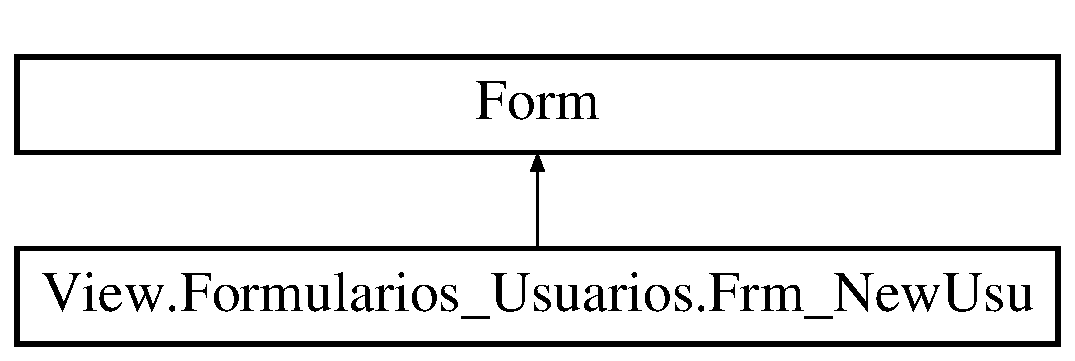
\includegraphics[height=2.000000cm]{class_view_1_1_formularios___usuarios_1_1_frm___new_usu}
\end{center}
\end{figure}
\subsection*{Membros protegidos}
\begin{DoxyCompactItemize}
\item 
override void \hyperlink{class_view_1_1_formularios___usuarios_1_1_frm___new_usu_af4dd878cfb325eda076a8a3b8f85fa9c}{Dispose} (bool disposing)
\begin{DoxyCompactList}\small\item\em Clean up any resources being used. \end{DoxyCompactList}\end{DoxyCompactItemize}


\subsection{Documentação dos métodos}
\hypertarget{class_view_1_1_formularios___usuarios_1_1_frm___new_usu_af4dd878cfb325eda076a8a3b8f85fa9c}{}\index{View\+::\+Formularios\+\_\+\+Usuarios\+::\+Frm\+\_\+\+New\+Usu@{View\+::\+Formularios\+\_\+\+Usuarios\+::\+Frm\+\_\+\+New\+Usu}!Dispose@{Dispose}}
\index{Dispose@{Dispose}!View\+::\+Formularios\+\_\+\+Usuarios\+::\+Frm\+\_\+\+New\+Usu@{View\+::\+Formularios\+\_\+\+Usuarios\+::\+Frm\+\_\+\+New\+Usu}}
\subsubsection[{Dispose(bool disposing)}]{\setlength{\rightskip}{0pt plus 5cm}override void View.\+Formularios\+\_\+\+Usuarios.\+Frm\+\_\+\+New\+Usu.\+Dispose (
\begin{DoxyParamCaption}
\item[{bool}]{disposing}
\end{DoxyParamCaption}
)\hspace{0.3cm}{\ttfamily [protected]}}\label{class_view_1_1_formularios___usuarios_1_1_frm___new_usu_af4dd878cfb325eda076a8a3b8f85fa9c}


Clean up any resources being used. 


\begin{DoxyParams}{Parâmetros}
{\em disposing} & true if managed resources should be disposed; otherwise, false.\\
\hline
\end{DoxyParams}


A documentação para esta classe foi gerada a partir dos seguintes ficheiros\+:\begin{DoxyCompactItemize}
\item 
D\+:/\+Projetos/\+Software\+Ordem\+De\+Servico/\+View/\+Usuario/Frm\+\_\+\+New\+Usu.\+cs\item 
D\+:/\+Projetos/\+Software\+Ordem\+De\+Servico/\+View/\+Usuario/Frm\+\_\+\+New\+Usu.\+Designer.\+cs\end{DoxyCompactItemize}

\hypertarget{class_view_1_1_opicoes_1_1_frm___opicoes_inicial}{}\section{Referência à classe View.\+Opicoes.\+Frm\+\_\+\+Opicoes\+Inicial}
\label{class_view_1_1_opicoes_1_1_frm___opicoes_inicial}\index{View.\+Opicoes.\+Frm\+\_\+\+Opicoes\+Inicial@{View.\+Opicoes.\+Frm\+\_\+\+Opicoes\+Inicial}}
Diagrama de heranças da classe View.\+Opicoes.\+Frm\+\_\+\+Opicoes\+Inicial\begin{figure}[H]
\begin{center}
\leavevmode
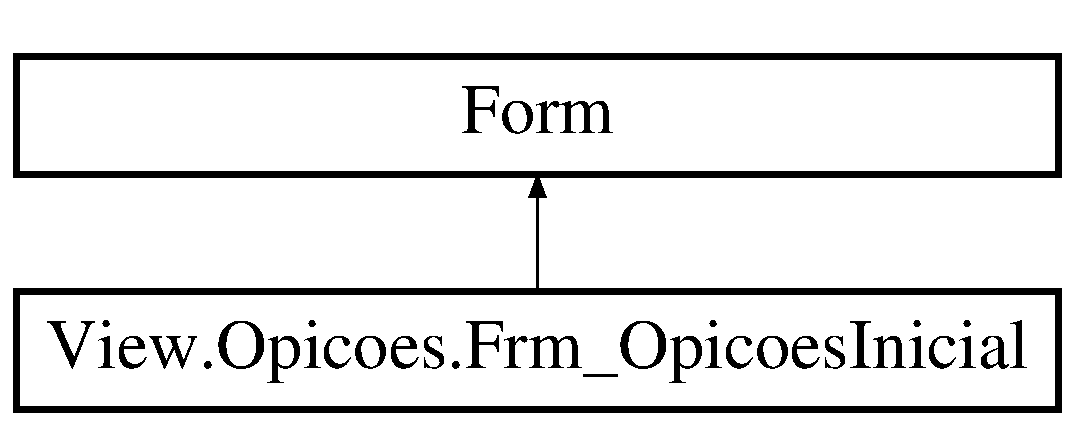
\includegraphics[height=2.000000cm]{class_view_1_1_opicoes_1_1_frm___opicoes_inicial}
\end{center}
\end{figure}
\subsection*{Membros protegidos}
\begin{DoxyCompactItemize}
\item 
override void \hyperlink{class_view_1_1_opicoes_1_1_frm___opicoes_inicial_a6eed7b80ed2a25991117eb29ef92bb24}{Dispose} (bool disposing)
\begin{DoxyCompactList}\small\item\em Clean up any resources being used. \end{DoxyCompactList}\end{DoxyCompactItemize}


\subsection{Documentação dos métodos}
\hypertarget{class_view_1_1_opicoes_1_1_frm___opicoes_inicial_a6eed7b80ed2a25991117eb29ef92bb24}{}\index{View\+::\+Opicoes\+::\+Frm\+\_\+\+Opicoes\+Inicial@{View\+::\+Opicoes\+::\+Frm\+\_\+\+Opicoes\+Inicial}!Dispose@{Dispose}}
\index{Dispose@{Dispose}!View\+::\+Opicoes\+::\+Frm\+\_\+\+Opicoes\+Inicial@{View\+::\+Opicoes\+::\+Frm\+\_\+\+Opicoes\+Inicial}}
\subsubsection[{Dispose(bool disposing)}]{\setlength{\rightskip}{0pt plus 5cm}override void View.\+Opicoes.\+Frm\+\_\+\+Opicoes\+Inicial.\+Dispose (
\begin{DoxyParamCaption}
\item[{bool}]{disposing}
\end{DoxyParamCaption}
)\hspace{0.3cm}{\ttfamily [protected]}}\label{class_view_1_1_opicoes_1_1_frm___opicoes_inicial_a6eed7b80ed2a25991117eb29ef92bb24}


Clean up any resources being used. 


\begin{DoxyParams}{Parâmetros}
{\em disposing} & true if managed resources should be disposed; otherwise, false.\\
\hline
\end{DoxyParams}


A documentação para esta classe foi gerada a partir dos seguintes ficheiros\+:\begin{DoxyCompactItemize}
\item 
C\+:/\+Cristiano/\+Projetos/\+Software\+Ordem\+De\+Servico/\+View/\+Opcoes/Frm\+\_\+\+Opicoes\+Inicial.\+cs\item 
C\+:/\+Cristiano/\+Projetos/\+Software\+Ordem\+De\+Servico/\+View/\+Opcoes/Frm\+\_\+\+Opicoes\+Inicial.\+Designer.\+cs\end{DoxyCompactItemize}

\hypertarget{class_view_1_1_frm___pai}{}\section{Referência à classe View.\+Frm\+\_\+\+Pai}
\label{class_view_1_1_frm___pai}\index{View.\+Frm\+\_\+\+Pai@{View.\+Frm\+\_\+\+Pai}}
Diagrama de heranças da classe View.\+Frm\+\_\+\+Pai\begin{figure}[H]
\begin{center}
\leavevmode
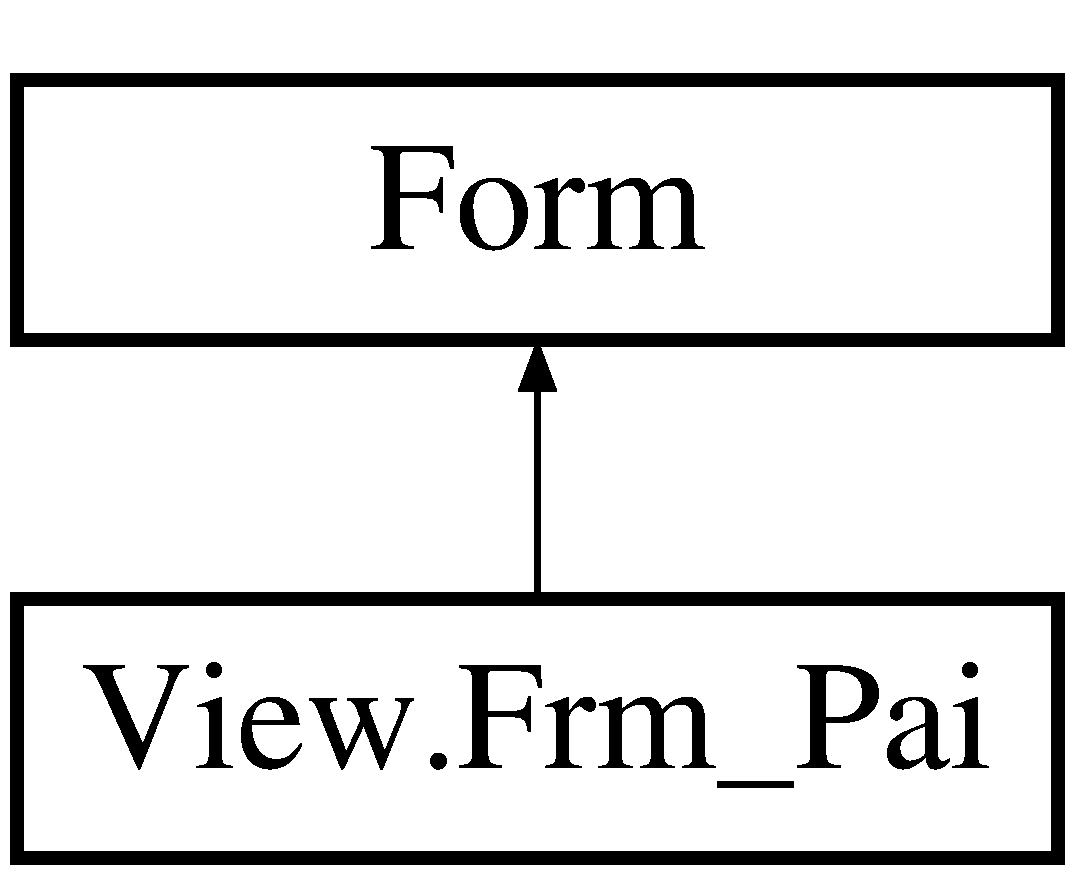
\includegraphics[height=2.000000cm]{class_view_1_1_frm___pai}
\end{center}
\end{figure}
\subsection*{Membros públicos}
\begin{DoxyCompactItemize}
\item 
\hypertarget{class_view_1_1_frm___pai_afc7f379d276cbd7eda18807237ca2168}{}{\bfseries Frm\+\_\+\+Pai} (string usuario, string nivel\+Acesso)\label{class_view_1_1_frm___pai_afc7f379d276cbd7eda18807237ca2168}

\end{DoxyCompactItemize}
\subsection*{Membros protegidos}
\begin{DoxyCompactItemize}
\item 
override void \hyperlink{class_view_1_1_frm___pai_a690f74bbe1f715ef71a1e3605d26a0fc}{Dispose} (bool disposing)
\begin{DoxyCompactList}\small\item\em Limpar os recursos que estão sendo usados. \end{DoxyCompactList}\end{DoxyCompactItemize}


\subsection{Documentação dos métodos}
\hypertarget{class_view_1_1_frm___pai_a690f74bbe1f715ef71a1e3605d26a0fc}{}\index{View\+::\+Frm\+\_\+\+Pai@{View\+::\+Frm\+\_\+\+Pai}!Dispose@{Dispose}}
\index{Dispose@{Dispose}!View\+::\+Frm\+\_\+\+Pai@{View\+::\+Frm\+\_\+\+Pai}}
\subsubsection[{Dispose(bool disposing)}]{\setlength{\rightskip}{0pt plus 5cm}override void View.\+Frm\+\_\+\+Pai.\+Dispose (
\begin{DoxyParamCaption}
\item[{bool}]{disposing}
\end{DoxyParamCaption}
)\hspace{0.3cm}{\ttfamily [protected]}}\label{class_view_1_1_frm___pai_a690f74bbe1f715ef71a1e3605d26a0fc}


Limpar os recursos que estão sendo usados. 


\begin{DoxyParams}{Parâmetros}
{\em disposing} & true se for necessário descartar os recursos gerenciados; caso contrário, false.\\
\hline
\end{DoxyParams}


A documentação para esta classe foi gerada a partir dos seguintes ficheiros\+:\begin{DoxyCompactItemize}
\item 
D\+:/\+Projetos/\+Software\+Ordem\+De\+Servico/\+View/\+Outros/Frm\+\_\+\+Pai.\+cs\item 
D\+:/\+Projetos/\+Software\+Ordem\+De\+Servico/\+View/\+Outros/Frm\+\_\+\+Pai.\+Designer.\+cs\end{DoxyCompactItemize}

\hypertarget{class_view_1_1_pessoas_1_1_frm___pessoa_fisica}{}\section{Referência à classe View.\+Pessoas.\+Frm\+\_\+\+Pessoa\+Fisica}
\label{class_view_1_1_pessoas_1_1_frm___pessoa_fisica}\index{View.\+Pessoas.\+Frm\+\_\+\+Pessoa\+Fisica@{View.\+Pessoas.\+Frm\+\_\+\+Pessoa\+Fisica}}
Diagrama de heranças da classe View.\+Pessoas.\+Frm\+\_\+\+Pessoa\+Fisica\begin{figure}[H]
\begin{center}
\leavevmode
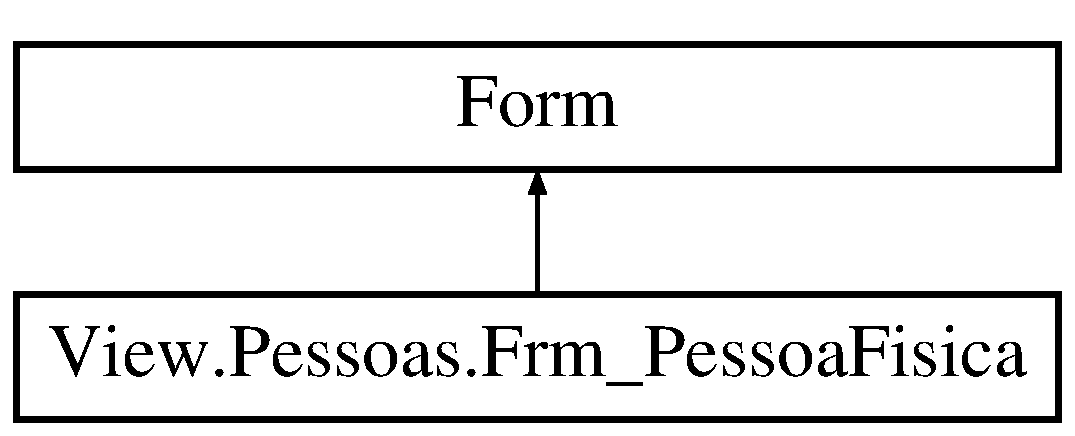
\includegraphics[height=2.000000cm]{class_view_1_1_pessoas_1_1_frm___pessoa_fisica}
\end{center}
\end{figure}
\subsection*{Membros protegidos}
\begin{DoxyCompactItemize}
\item 
override void \hyperlink{class_view_1_1_pessoas_1_1_frm___pessoa_fisica_a67b75d50b70a4be7f9b39b9a8c7ee00d}{Dispose} (bool disposing)
\begin{DoxyCompactList}\small\item\em Clean up any resources being used. \end{DoxyCompactList}\end{DoxyCompactItemize}


\subsection{Documentação dos métodos}
\hypertarget{class_view_1_1_pessoas_1_1_frm___pessoa_fisica_a67b75d50b70a4be7f9b39b9a8c7ee00d}{}\index{View\+::\+Pessoas\+::\+Frm\+\_\+\+Pessoa\+Fisica@{View\+::\+Pessoas\+::\+Frm\+\_\+\+Pessoa\+Fisica}!Dispose@{Dispose}}
\index{Dispose@{Dispose}!View\+::\+Pessoas\+::\+Frm\+\_\+\+Pessoa\+Fisica@{View\+::\+Pessoas\+::\+Frm\+\_\+\+Pessoa\+Fisica}}
\subsubsection[{Dispose(bool disposing)}]{\setlength{\rightskip}{0pt plus 5cm}override void View.\+Pessoas.\+Frm\+\_\+\+Pessoa\+Fisica.\+Dispose (
\begin{DoxyParamCaption}
\item[{bool}]{disposing}
\end{DoxyParamCaption}
)\hspace{0.3cm}{\ttfamily [protected]}}\label{class_view_1_1_pessoas_1_1_frm___pessoa_fisica_a67b75d50b70a4be7f9b39b9a8c7ee00d}


Clean up any resources being used. 


\begin{DoxyParams}{Parâmetros}
{\em disposing} & true if managed resources should be disposed; otherwise, false.\\
\hline
\end{DoxyParams}


A documentação para esta classe foi gerada a partir dos seguintes ficheiros\+:\begin{DoxyCompactItemize}
\item 
D\+:/\+Projetos/\+Software\+Ordem\+De\+Servico/\+View/\+Pessoas/Frm\+\_\+\+Pessoa\+Fisica.\+cs\item 
D\+:/\+Projetos/\+Software\+Ordem\+De\+Servico/\+View/\+Pessoas/Frm\+\_\+\+Pessoa\+Fisica.\+Designer.\+cs\end{DoxyCompactItemize}

\hypertarget{class_view_1_1_pessoas_1_1_frm___pessoa_juridica}{}\section{Referência à classe View.\+Pessoas.\+Frm\+\_\+\+Pessoa\+Juridica}
\label{class_view_1_1_pessoas_1_1_frm___pessoa_juridica}\index{View.\+Pessoas.\+Frm\+\_\+\+Pessoa\+Juridica@{View.\+Pessoas.\+Frm\+\_\+\+Pessoa\+Juridica}}
Diagrama de heranças da classe View.\+Pessoas.\+Frm\+\_\+\+Pessoa\+Juridica\begin{figure}[H]
\begin{center}
\leavevmode
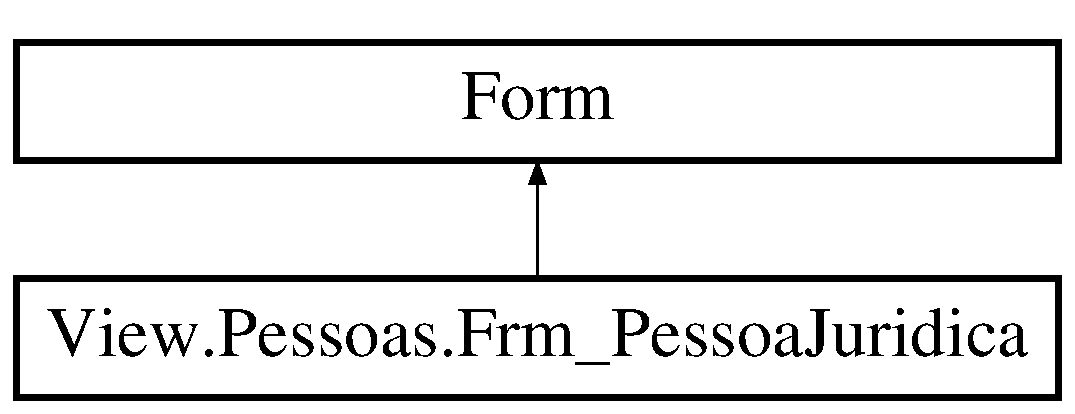
\includegraphics[height=2.000000cm]{class_view_1_1_pessoas_1_1_frm___pessoa_juridica}
\end{center}
\end{figure}
\subsection*{Membros protegidos}
\begin{DoxyCompactItemize}
\item 
override void \hyperlink{class_view_1_1_pessoas_1_1_frm___pessoa_juridica_a39fb51213737a31e69dd30f9237df9d2}{Dispose} (bool disposing)
\begin{DoxyCompactList}\small\item\em Clean up any resources being used. \end{DoxyCompactList}\end{DoxyCompactItemize}


\subsection{Documentação dos métodos}
\hypertarget{class_view_1_1_pessoas_1_1_frm___pessoa_juridica_a39fb51213737a31e69dd30f9237df9d2}{}\index{View\+::\+Pessoas\+::\+Frm\+\_\+\+Pessoa\+Juridica@{View\+::\+Pessoas\+::\+Frm\+\_\+\+Pessoa\+Juridica}!Dispose@{Dispose}}
\index{Dispose@{Dispose}!View\+::\+Pessoas\+::\+Frm\+\_\+\+Pessoa\+Juridica@{View\+::\+Pessoas\+::\+Frm\+\_\+\+Pessoa\+Juridica}}
\subsubsection[{Dispose(bool disposing)}]{\setlength{\rightskip}{0pt plus 5cm}override void View.\+Pessoas.\+Frm\+\_\+\+Pessoa\+Juridica.\+Dispose (
\begin{DoxyParamCaption}
\item[{bool}]{disposing}
\end{DoxyParamCaption}
)\hspace{0.3cm}{\ttfamily [protected]}}\label{class_view_1_1_pessoas_1_1_frm___pessoa_juridica_a39fb51213737a31e69dd30f9237df9d2}


Clean up any resources being used. 


\begin{DoxyParams}{Parâmetros}
{\em disposing} & true if managed resources should be disposed; otherwise, false.\\
\hline
\end{DoxyParams}


A documentação para esta classe foi gerada a partir dos seguintes ficheiros\+:\begin{DoxyCompactItemize}
\item 
C\+:/\+Cristiano/\+Projetos/\+Software\+Ordem\+De\+Servico/\+View/\+Pessoas/Frm\+\_\+\+Pessoa\+Juridica.\+cs\item 
C\+:/\+Cristiano/\+Projetos/\+Software\+Ordem\+De\+Servico/\+View/\+Pessoas/Frm\+\_\+\+Pessoa\+Juridica.\+Designer.\+cs\end{DoxyCompactItemize}

\hypertarget{class_view_1_1_outros_1_1_frm___sobre}{}\section{Referência à classe View.\+Outros.\+Frm\+\_\+\+Sobre}
\label{class_view_1_1_outros_1_1_frm___sobre}\index{View.\+Outros.\+Frm\+\_\+\+Sobre@{View.\+Outros.\+Frm\+\_\+\+Sobre}}
Diagrama de heranças da classe View.\+Outros.\+Frm\+\_\+\+Sobre\begin{figure}[H]
\begin{center}
\leavevmode
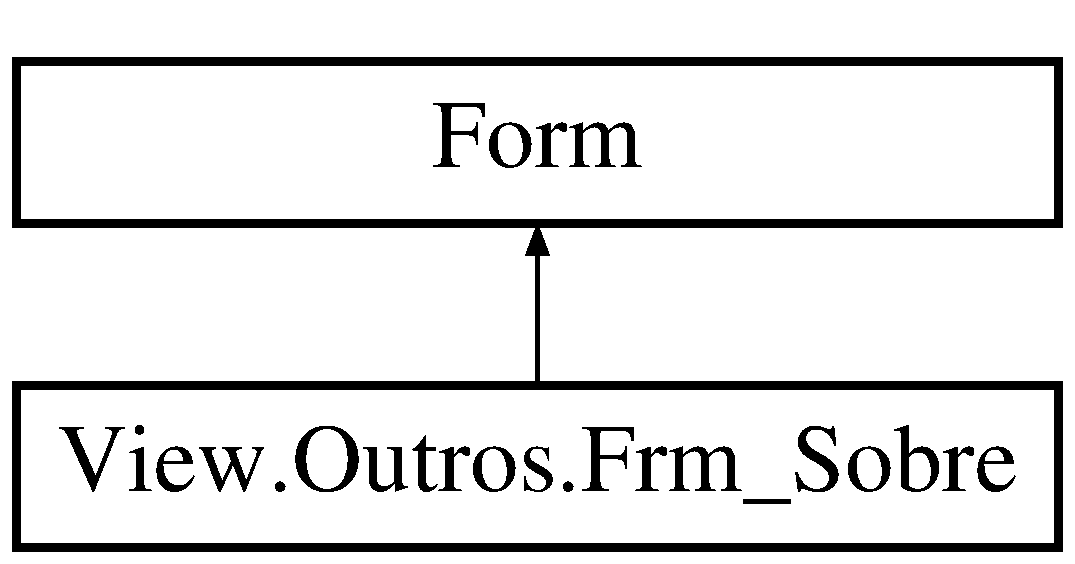
\includegraphics[height=2.000000cm]{class_view_1_1_outros_1_1_frm___sobre}
\end{center}
\end{figure}
\subsection*{Membros protegidos}
\begin{DoxyCompactItemize}
\item 
override void \hyperlink{class_view_1_1_outros_1_1_frm___sobre_ae508ccd5e120c0e538c60a89cd4cdf16}{Dispose} (bool disposing)
\begin{DoxyCompactList}\small\item\em Limpar os recursos que estão sendo usados. \end{DoxyCompactList}\end{DoxyCompactItemize}
\subsection*{Propriedades}
\begin{DoxyCompactItemize}
\item 
\hypertarget{class_view_1_1_outros_1_1_frm___sobre_a30862d942844e1cc9200426b10567265}{}string {\bfseries Assembly\+Title}\hspace{0.3cm}{\ttfamily  \mbox{[}get\mbox{]}}\label{class_view_1_1_outros_1_1_frm___sobre_a30862d942844e1cc9200426b10567265}

\item 
\hypertarget{class_view_1_1_outros_1_1_frm___sobre_a71ff2eed7b5d3a9d33b03c32d45cbb02}{}string {\bfseries Assembly\+Version}\hspace{0.3cm}{\ttfamily  \mbox{[}get\mbox{]}}\label{class_view_1_1_outros_1_1_frm___sobre_a71ff2eed7b5d3a9d33b03c32d45cbb02}

\item 
\hypertarget{class_view_1_1_outros_1_1_frm___sobre_a8dce575534a194e1f25e889c13c7d719}{}string {\bfseries Assembly\+Description}\hspace{0.3cm}{\ttfamily  \mbox{[}get\mbox{]}}\label{class_view_1_1_outros_1_1_frm___sobre_a8dce575534a194e1f25e889c13c7d719}

\item 
\hypertarget{class_view_1_1_outros_1_1_frm___sobre_ab2b4377ad47af889b02e67921581d346}{}string {\bfseries Assembly\+Product}\hspace{0.3cm}{\ttfamily  \mbox{[}get\mbox{]}}\label{class_view_1_1_outros_1_1_frm___sobre_ab2b4377ad47af889b02e67921581d346}

\item 
\hypertarget{class_view_1_1_outros_1_1_frm___sobre_afed0773db8b9c0492e1756540f9feb79}{}string {\bfseries Assembly\+Copyright}\hspace{0.3cm}{\ttfamily  \mbox{[}get\mbox{]}}\label{class_view_1_1_outros_1_1_frm___sobre_afed0773db8b9c0492e1756540f9feb79}

\item 
\hypertarget{class_view_1_1_outros_1_1_frm___sobre_a8433fa0603c17182376a7cbdc655f4a2}{}string {\bfseries Assembly\+Company}\hspace{0.3cm}{\ttfamily  \mbox{[}get\mbox{]}}\label{class_view_1_1_outros_1_1_frm___sobre_a8433fa0603c17182376a7cbdc655f4a2}

\end{DoxyCompactItemize}


\subsection{Documentação dos métodos}
\hypertarget{class_view_1_1_outros_1_1_frm___sobre_ae508ccd5e120c0e538c60a89cd4cdf16}{}\index{View\+::\+Outros\+::\+Frm\+\_\+\+Sobre@{View\+::\+Outros\+::\+Frm\+\_\+\+Sobre}!Dispose@{Dispose}}
\index{Dispose@{Dispose}!View\+::\+Outros\+::\+Frm\+\_\+\+Sobre@{View\+::\+Outros\+::\+Frm\+\_\+\+Sobre}}
\subsubsection[{Dispose(bool disposing)}]{\setlength{\rightskip}{0pt plus 5cm}override void View.\+Outros.\+Frm\+\_\+\+Sobre.\+Dispose (
\begin{DoxyParamCaption}
\item[{bool}]{disposing}
\end{DoxyParamCaption}
)\hspace{0.3cm}{\ttfamily [protected]}}\label{class_view_1_1_outros_1_1_frm___sobre_ae508ccd5e120c0e538c60a89cd4cdf16}


Limpar os recursos que estão sendo usados. 



A documentação para esta classe foi gerada a partir dos seguintes ficheiros\+:\begin{DoxyCompactItemize}
\item 
D\+:/\+Projetos/\+Software\+Ordem\+De\+Servico/\+View/\+Outros/Frm\+\_\+\+Sobre.\+cs\item 
D\+:/\+Projetos/\+Software\+Ordem\+De\+Servico/\+View/\+Outros/Frm\+\_\+\+Sobre.\+Designer.\+cs\end{DoxyCompactItemize}

\hypertarget{class_model_1_1_pessoa__e___usuario_1_1_juridica}{}\section{Referência à classe Model.\+Pessoa\+\_\+e\+\_\+\+Usuario.\+Juridica}
\label{class_model_1_1_pessoa__e___usuario_1_1_juridica}\index{Model.\+Pessoa\+\_\+e\+\_\+\+Usuario.\+Juridica@{Model.\+Pessoa\+\_\+e\+\_\+\+Usuario.\+Juridica}}
Diagrama de heranças da classe Model.\+Pessoa\+\_\+e\+\_\+\+Usuario.\+Juridica\begin{figure}[H]
\begin{center}
\leavevmode
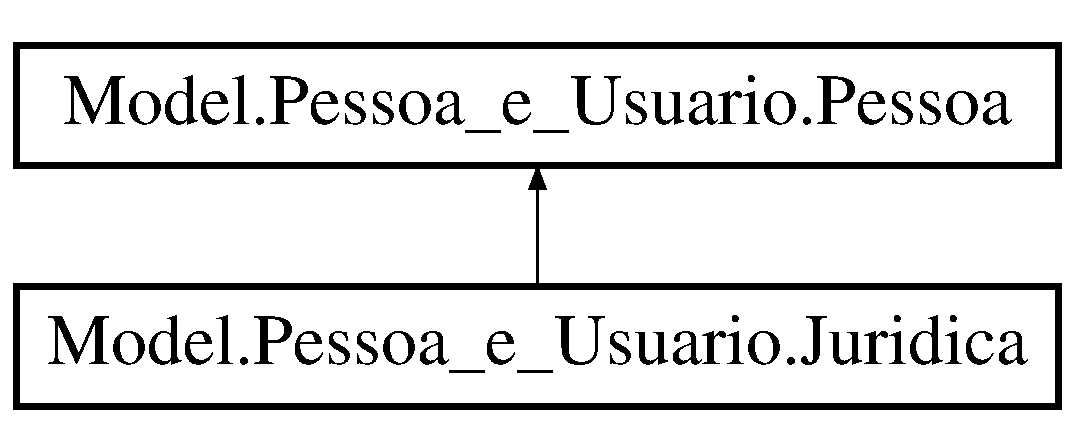
\includegraphics[height=2.000000cm]{class_model_1_1_pessoa__e___usuario_1_1_juridica}
\end{center}
\end{figure}
\subsection*{Membros públicos}
\begin{DoxyCompactItemize}
\item 
String \hyperlink{class_model_1_1_pessoa__e___usuario_1_1_juridica_aa6276e88b7f8ebfdeba461d011d264a7}{Save} (string \+\_\+nome, string \+\_\+endereco, string \+\_\+telefone, string \+\_\+situacao, string \+\_\+sigla\+Estado, string \+\_\+cidade, string \+\_\+bairro, string \+\_\+cep, string \+\_\+observacoes, string \+\_\+cnpj, string \+\_\+contato, string \+\_\+inscricaoestadual, string \+\_\+razaosocial)
\begin{DoxyCompactList}\small\item\em Salvando pessoa Jurídica na pasta \char`\"{}\+J\char`\"{}(Pasta usada para guardar todas as pessoas jurídicas no diretorio do software) \end{DoxyCompactList}\item 
\hyperlink{class_model_1_1_pessoa__e___usuario_1_1_juridica}{Juridica} \hyperlink{class_model_1_1_pessoa__e___usuario_1_1_juridica_a0178595c1d5df0fa74712c465f469345}{Load} (String \+\_\+\+Identificador\+Load)
\begin{DoxyCompactList}\small\item\em Carregando pessoa Física. \end{DoxyCompactList}\item 
List$<$ string $>$ \hyperlink{class_model_1_1_pessoa__e___usuario_1_1_juridica_ac7b5ac912bb65ee21b26ef2c99cc5123}{Load\+List} ()
\begin{DoxyCompactList}\small\item\em Carregando Lista com nome de todas pessoas Jurídicas registradas. \end{DoxyCompactList}\item 
bool \hyperlink{class_model_1_1_pessoa__e___usuario_1_1_juridica_a01755510e8044733c5a795804bd11523}{Verificar} (String \+\_\+nome)
\begin{DoxyCompactList}\small\item\em Verificando de a \char`\"{}\+Pessoa jurídica\char`\"{} existe. \end{DoxyCompactList}\end{DoxyCompactItemize}
\subsection*{Propriedades}
\begin{DoxyCompactItemize}
\item 
\hypertarget{class_model_1_1_pessoa__e___usuario_1_1_juridica_a51ed47e7767ea639a4631811968b2917}{}string {\bfseries Razao\+Social}\hspace{0.3cm}{\ttfamily  \mbox{[}get, set\mbox{]}}\label{class_model_1_1_pessoa__e___usuario_1_1_juridica_a51ed47e7767ea639a4631811968b2917}

\item 
\hypertarget{class_model_1_1_pessoa__e___usuario_1_1_juridica_a56cf8933a76cdc033f957eb2863963b7}{}string {\bfseries Cnpj}\hspace{0.3cm}{\ttfamily  \mbox{[}get, set\mbox{]}}\label{class_model_1_1_pessoa__e___usuario_1_1_juridica_a56cf8933a76cdc033f957eb2863963b7}

\item 
\hypertarget{class_model_1_1_pessoa__e___usuario_1_1_juridica_a284c0f5d214e60939d8418c793ca798d}{}string {\bfseries Contato}\hspace{0.3cm}{\ttfamily  \mbox{[}get, set\mbox{]}}\label{class_model_1_1_pessoa__e___usuario_1_1_juridica_a284c0f5d214e60939d8418c793ca798d}

\item 
\hypertarget{class_model_1_1_pessoa__e___usuario_1_1_juridica_ae9b2c1e10ba35a555be2991a8b18892f}{}string {\bfseries Inscricao\+Estadual}\hspace{0.3cm}{\ttfamily  \mbox{[}get, set\mbox{]}}\label{class_model_1_1_pessoa__e___usuario_1_1_juridica_ae9b2c1e10ba35a555be2991a8b18892f}

\end{DoxyCompactItemize}


\subsection{Documentação dos métodos}
\hypertarget{class_model_1_1_pessoa__e___usuario_1_1_juridica_a0178595c1d5df0fa74712c465f469345}{}\index{Model\+::\+Pessoa\+\_\+e\+\_\+\+Usuario\+::\+Juridica@{Model\+::\+Pessoa\+\_\+e\+\_\+\+Usuario\+::\+Juridica}!Load@{Load}}
\index{Load@{Load}!Model\+::\+Pessoa\+\_\+e\+\_\+\+Usuario\+::\+Juridica@{Model\+::\+Pessoa\+\_\+e\+\_\+\+Usuario\+::\+Juridica}}
\subsubsection[{Load(\+String \+\_\+\+Identificador\+Load)}]{\setlength{\rightskip}{0pt plus 5cm}{\bf Juridica} Model.\+Pessoa\+\_\+e\+\_\+\+Usuario.\+Juridica.\+Load (
\begin{DoxyParamCaption}
\item[{String}]{\+\_\+\+Identificador\+Load}
\end{DoxyParamCaption}
)}\label{class_model_1_1_pessoa__e___usuario_1_1_juridica_a0178595c1d5df0fa74712c465f469345}


Carregando pessoa Física. 


\begin{DoxyParams}{Parâmetros}
{\em \+\_\+\+Identificador\+Load} & \\
\hline
\end{DoxyParams}
\begin{DoxyReturn}{Retorna}
\hyperlink{class_model_1_1_pessoa__e___usuario_1_1_pessoa}{Pessoa} Jurídica.
\end{DoxyReturn}
\hypertarget{class_model_1_1_pessoa__e___usuario_1_1_juridica_ac7b5ac912bb65ee21b26ef2c99cc5123}{}\index{Model\+::\+Pessoa\+\_\+e\+\_\+\+Usuario\+::\+Juridica@{Model\+::\+Pessoa\+\_\+e\+\_\+\+Usuario\+::\+Juridica}!Load\+List@{Load\+List}}
\index{Load\+List@{Load\+List}!Model\+::\+Pessoa\+\_\+e\+\_\+\+Usuario\+::\+Juridica@{Model\+::\+Pessoa\+\_\+e\+\_\+\+Usuario\+::\+Juridica}}
\subsubsection[{Load\+List()}]{\setlength{\rightskip}{0pt plus 5cm}List$<$string$>$ Model.\+Pessoa\+\_\+e\+\_\+\+Usuario.\+Juridica.\+Load\+List (
\begin{DoxyParamCaption}
{}
\end{DoxyParamCaption}
)}\label{class_model_1_1_pessoa__e___usuario_1_1_juridica_ac7b5ac912bb65ee21b26ef2c99cc5123}


Carregando Lista com nome de todas pessoas Jurídicas registradas. 

\begin{DoxyReturn}{Retorna}
Lista de nomes.
\end{DoxyReturn}
\hypertarget{class_model_1_1_pessoa__e___usuario_1_1_juridica_aa6276e88b7f8ebfdeba461d011d264a7}{}\index{Model\+::\+Pessoa\+\_\+e\+\_\+\+Usuario\+::\+Juridica@{Model\+::\+Pessoa\+\_\+e\+\_\+\+Usuario\+::\+Juridica}!Save@{Save}}
\index{Save@{Save}!Model\+::\+Pessoa\+\_\+e\+\_\+\+Usuario\+::\+Juridica@{Model\+::\+Pessoa\+\_\+e\+\_\+\+Usuario\+::\+Juridica}}
\subsubsection[{Save(string \+\_\+nome, string \+\_\+endereco, string \+\_\+telefone, string \+\_\+situacao, string \+\_\+sigla\+Estado, string \+\_\+cidade, string \+\_\+bairro, string \+\_\+cep, string \+\_\+observacoes, string \+\_\+cnpj, string \+\_\+contato, string \+\_\+inscricaoestadual, string \+\_\+razaosocial)}]{\setlength{\rightskip}{0pt plus 5cm}String Model.\+Pessoa\+\_\+e\+\_\+\+Usuario.\+Juridica.\+Save (
\begin{DoxyParamCaption}
\item[{string}]{\+\_\+nome, }
\item[{string}]{\+\_\+endereco, }
\item[{string}]{\+\_\+telefone, }
\item[{string}]{\+\_\+situacao, }
\item[{string}]{\+\_\+sigla\+Estado, }
\item[{string}]{\+\_\+cidade, }
\item[{string}]{\+\_\+bairro, }
\item[{string}]{\+\_\+cep, }
\item[{string}]{\+\_\+observacoes, }
\item[{string}]{\+\_\+cnpj, }
\item[{string}]{\+\_\+contato, }
\item[{string}]{\+\_\+inscricaoestadual, }
\item[{string}]{\+\_\+razaosocial}
\end{DoxyParamCaption}
)}\label{class_model_1_1_pessoa__e___usuario_1_1_juridica_aa6276e88b7f8ebfdeba461d011d264a7}


Salvando pessoa Jurídica na pasta \char`\"{}\+J\char`\"{}(Pasta usada para guardar todas as pessoas jurídicas no diretorio do software) 


\begin{DoxyParams}{Parâmetros}
{\em \+\_\+nome} & \\
\hline
{\em \+\_\+endereco} & \\
\hline
{\em \+\_\+telefone} & \\
\hline
{\em \+\_\+situacao} & \\
\hline
{\em \+\_\+sigla\+Estado} & \\
\hline
{\em \+\_\+cidade} & \\
\hline
{\em \+\_\+bairro} & \\
\hline
{\em \+\_\+cep} & \\
\hline
{\em \+\_\+observacoes} & \\
\hline
{\em \+\_\+cnpj} & \\
\hline
{\em \+\_\+contato} & \\
\hline
{\em \+\_\+inscricaoestadual} & \\
\hline
{\em \+\_\+razaosocial} & \\
\hline
\end{DoxyParams}
\begin{DoxyReturn}{Retorna}

\end{DoxyReturn}
\hypertarget{class_model_1_1_pessoa__e___usuario_1_1_juridica_a01755510e8044733c5a795804bd11523}{}\index{Model\+::\+Pessoa\+\_\+e\+\_\+\+Usuario\+::\+Juridica@{Model\+::\+Pessoa\+\_\+e\+\_\+\+Usuario\+::\+Juridica}!Verificar@{Verificar}}
\index{Verificar@{Verificar}!Model\+::\+Pessoa\+\_\+e\+\_\+\+Usuario\+::\+Juridica@{Model\+::\+Pessoa\+\_\+e\+\_\+\+Usuario\+::\+Juridica}}
\subsubsection[{Verificar(\+String \+\_\+nome)}]{\setlength{\rightskip}{0pt plus 5cm}bool Model.\+Pessoa\+\_\+e\+\_\+\+Usuario.\+Juridica.\+Verificar (
\begin{DoxyParamCaption}
\item[{String}]{\+\_\+nome}
\end{DoxyParamCaption}
)}\label{class_model_1_1_pessoa__e___usuario_1_1_juridica_a01755510e8044733c5a795804bd11523}


Verificando de a \char`\"{}\+Pessoa jurídica\char`\"{} existe. 


\begin{DoxyParams}{Parâmetros}
{\em \+\_\+nome} & \\
\hline
\end{DoxyParams}
\begin{DoxyReturn}{Retorna}

\end{DoxyReturn}


A documentação para esta classe foi gerada a partir do seguinte ficheiro\+:\begin{DoxyCompactItemize}
\item 
D\+:/\+Projetos/\+Software\+Ordem\+De\+Servico/\+Model/\+Pessoa e Usuario/Juridica.\+cs\end{DoxyCompactItemize}

\hypertarget{class_model_1_1_ordem__de___servico_1_1_ordem_servico}{}\section{Referência à classe Model.\+Ordem\+\_\+de\+\_\+\+Servico.\+Ordem\+Servico}
\label{class_model_1_1_ordem__de___servico_1_1_ordem_servico}\index{Model.\+Ordem\+\_\+de\+\_\+\+Servico.\+Ordem\+Servico@{Model.\+Ordem\+\_\+de\+\_\+\+Servico.\+Ordem\+Servico}}
\subsection*{Membros públicos}
\begin{DoxyCompactItemize}
\item 
void \hyperlink{class_model_1_1_ordem__de___servico_1_1_ordem_servico_aa2063b330d10dd34cffe6b354c5587fc}{Creat\+P\+D\+F} (string Identificador, string Referencia, string Situacao, string Defeito, string Descricao, string Observacao, string Numero\+Serie, string Equipamento, string Data\+Entrada\+Servico, string Cliente)
\begin{DoxyCompactList}\small\item\em Gerando P\+D\+F da ordem de serviço. (A ordem de serviço em P\+D\+F não fica salvar ela é gerada cada vez que a função é chamada) \end{DoxyCompactList}\item 
string \hyperlink{class_model_1_1_ordem__de___servico_1_1_ordem_servico_a098688c9491c28d72a3eba5dc9be5f89}{Save} (string Identificador, string Referencia, string Situacao, string Defeito, string Descricao, string Observacao, string Numero\+Serie, string Equipamento, string Data\+Entrada\+Servico, string Cliente)
\begin{DoxyCompactList}\small\item\em Salvando a ordem de serviço em arquivo de Texto. \end{DoxyCompactList}\item 
string \hyperlink{class_model_1_1_ordem__de___servico_1_1_ordem_servico_a7fe5d0e2c821d51a6bca866c1e861495}{Edit} (string Identificador, string Referencia, string Situacao, string Defeito, string Descricao, string Observacao, string Numero\+Serie, string Equipamento, string Data\+Entrada\+Servico, string Cliente)
\begin{DoxyCompactList}\small\item\em Editar a ordem de serviço, quase a mesam coisa que a \hyperlink{class_model_1_1_ordem__de___servico_1_1_ordem_servico_a098688c9491c28d72a3eba5dc9be5f89}{Save()}, ela só não verifica se o arquivo já existe, apenas salva. \end{DoxyCompactList}\item 
\hyperlink{class_model_1_1_ordem__de___servico_1_1_ordem_servico}{Ordem\+Servico} \hyperlink{class_model_1_1_ordem__de___servico_1_1_ordem_servico_a95c474e94611ca6f442866080dc19989}{Load} (string \+\_\+\+Identificador)
\begin{DoxyCompactList}\small\item\em Carregando a ordem de serviço atraves do arquivo de texto. \end{DoxyCompactList}\item 
List$<$ string $>$ \hyperlink{class_model_1_1_ordem__de___servico_1_1_ordem_servico_ae03ea1385455c47aa9adf39ab00fd72b}{Load\+List} ()
\begin{DoxyCompactList}\small\item\em Carrega uma lista de ordens de serviço. \end{DoxyCompactList}\item 
bool \hyperlink{class_model_1_1_ordem__de___servico_1_1_ordem_servico_a7959729db61c05f75261ce288e579ec2}{Verificar} (string \+\_\+\+Identificador)
\begin{DoxyCompactList}\small\item\em Verifica se a ordem de serviço existe ou não. \end{DoxyCompactList}\end{DoxyCompactItemize}
\subsection*{Propriedades}
\begin{DoxyCompactItemize}
\item 
\hypertarget{class_model_1_1_ordem__de___servico_1_1_ordem_servico_ab50cb47945c4c86c9b42aba5aece7000}{}string {\bfseries Identificador}\hspace{0.3cm}{\ttfamily  \mbox{[}get, set\mbox{]}}\label{class_model_1_1_ordem__de___servico_1_1_ordem_servico_ab50cb47945c4c86c9b42aba5aece7000}

\item 
\hypertarget{class_model_1_1_ordem__de___servico_1_1_ordem_servico_af054814a04f8a8d3a84865844837ffc9}{}string {\bfseries Referencia}\hspace{0.3cm}{\ttfamily  \mbox{[}get, set\mbox{]}}\label{class_model_1_1_ordem__de___servico_1_1_ordem_servico_af054814a04f8a8d3a84865844837ffc9}

\item 
\hypertarget{class_model_1_1_ordem__de___servico_1_1_ordem_servico_a3d0c97e6fe6180fa3d04e52352c38a75}{}string {\bfseries Situacao}\hspace{0.3cm}{\ttfamily  \mbox{[}get, set\mbox{]}}\label{class_model_1_1_ordem__de___servico_1_1_ordem_servico_a3d0c97e6fe6180fa3d04e52352c38a75}

\item 
\hypertarget{class_model_1_1_ordem__de___servico_1_1_ordem_servico_a29fafb8a6aee0c8cdc64f4e1a26398f9}{}string {\bfseries Defeito}\hspace{0.3cm}{\ttfamily  \mbox{[}get, set\mbox{]}}\label{class_model_1_1_ordem__de___servico_1_1_ordem_servico_a29fafb8a6aee0c8cdc64f4e1a26398f9}

\item 
\hypertarget{class_model_1_1_ordem__de___servico_1_1_ordem_servico_a0d34b506782f579945bad83a4c61e656}{}string {\bfseries Descricao}\hspace{0.3cm}{\ttfamily  \mbox{[}get, set\mbox{]}}\label{class_model_1_1_ordem__de___servico_1_1_ordem_servico_a0d34b506782f579945bad83a4c61e656}

\item 
\hypertarget{class_model_1_1_ordem__de___servico_1_1_ordem_servico_a3c3f7418d927ddc71abb008443979a3a}{}string {\bfseries Observacao}\hspace{0.3cm}{\ttfamily  \mbox{[}get, set\mbox{]}}\label{class_model_1_1_ordem__de___servico_1_1_ordem_servico_a3c3f7418d927ddc71abb008443979a3a}

\item 
\hypertarget{class_model_1_1_ordem__de___servico_1_1_ordem_servico_a0969417157e2d0e2438858dd4568ab6c}{}string {\bfseries Numero\+Serie}\hspace{0.3cm}{\ttfamily  \mbox{[}get, set\mbox{]}}\label{class_model_1_1_ordem__de___servico_1_1_ordem_servico_a0969417157e2d0e2438858dd4568ab6c}

\item 
\hypertarget{class_model_1_1_ordem__de___servico_1_1_ordem_servico_a671dafafad5d1da8afa821d0227f781c}{}string {\bfseries Equipamento}\hspace{0.3cm}{\ttfamily  \mbox{[}get, set\mbox{]}}\label{class_model_1_1_ordem__de___servico_1_1_ordem_servico_a671dafafad5d1da8afa821d0227f781c}

\item 
\hypertarget{class_model_1_1_ordem__de___servico_1_1_ordem_servico_a5eeebe5356f0a238ad1c8955bbde8beb}{}string {\bfseries Data\+Entrada\+Servico}\hspace{0.3cm}{\ttfamily  \mbox{[}get, set\mbox{]}}\label{class_model_1_1_ordem__de___servico_1_1_ordem_servico_a5eeebe5356f0a238ad1c8955bbde8beb}

\item 
\hypertarget{class_model_1_1_ordem__de___servico_1_1_ordem_servico_afbbda50a1d9541535e5e68ec231de5e9}{}string {\bfseries Cliente}\hspace{0.3cm}{\ttfamily  \mbox{[}get, set\mbox{]}}\label{class_model_1_1_ordem__de___servico_1_1_ordem_servico_afbbda50a1d9541535e5e68ec231de5e9}

\end{DoxyCompactItemize}


\subsection{Documentação dos métodos}
\hypertarget{class_model_1_1_ordem__de___servico_1_1_ordem_servico_aa2063b330d10dd34cffe6b354c5587fc}{}\index{Model\+::\+Ordem\+\_\+de\+\_\+\+Servico\+::\+Ordem\+Servico@{Model\+::\+Ordem\+\_\+de\+\_\+\+Servico\+::\+Ordem\+Servico}!Creat\+P\+D\+F@{Creat\+P\+D\+F}}
\index{Creat\+P\+D\+F@{Creat\+P\+D\+F}!Model\+::\+Ordem\+\_\+de\+\_\+\+Servico\+::\+Ordem\+Servico@{Model\+::\+Ordem\+\_\+de\+\_\+\+Servico\+::\+Ordem\+Servico}}
\subsubsection[{Creat\+P\+D\+F(string Identificador, string Referencia, string Situacao, string Defeito, string Descricao, string Observacao, string Numero\+Serie, string Equipamento, string Data\+Entrada\+Servico, string Cliente)}]{\setlength{\rightskip}{0pt plus 5cm}void Model.\+Ordem\+\_\+de\+\_\+\+Servico.\+Ordem\+Servico.\+Creat\+P\+D\+F (
\begin{DoxyParamCaption}
\item[{string}]{Identificador, }
\item[{string}]{Referencia, }
\item[{string}]{Situacao, }
\item[{string}]{Defeito, }
\item[{string}]{Descricao, }
\item[{string}]{Observacao, }
\item[{string}]{Numero\+Serie, }
\item[{string}]{Equipamento, }
\item[{string}]{Data\+Entrada\+Servico, }
\item[{string}]{Cliente}
\end{DoxyParamCaption}
)}\label{class_model_1_1_ordem__de___servico_1_1_ordem_servico_aa2063b330d10dd34cffe6b354c5587fc}


Gerando P\+D\+F da ordem de serviço. (A ordem de serviço em P\+D\+F não fica salvar ela é gerada cada vez que a função é chamada) 


\begin{DoxyParams}{Parâmetros}
{\em Identificador} & \\
\hline
{\em Referencia} & \\
\hline
{\em Situacao} & \\
\hline
{\em Defeito} & \\
\hline
{\em Descricao} & \\
\hline
{\em Observacao} & \\
\hline
{\em Numero\+Serie} & \\
\hline
{\em Equipamento} & \\
\hline
{\em Data\+Entrada\+Servico} & \\
\hline
{\em Cliente} & \\
\hline
\end{DoxyParams}
\hypertarget{class_model_1_1_ordem__de___servico_1_1_ordem_servico_a7fe5d0e2c821d51a6bca866c1e861495}{}\index{Model\+::\+Ordem\+\_\+de\+\_\+\+Servico\+::\+Ordem\+Servico@{Model\+::\+Ordem\+\_\+de\+\_\+\+Servico\+::\+Ordem\+Servico}!Edit@{Edit}}
\index{Edit@{Edit}!Model\+::\+Ordem\+\_\+de\+\_\+\+Servico\+::\+Ordem\+Servico@{Model\+::\+Ordem\+\_\+de\+\_\+\+Servico\+::\+Ordem\+Servico}}
\subsubsection[{Edit(string Identificador, string Referencia, string Situacao, string Defeito, string Descricao, string Observacao, string Numero\+Serie, string Equipamento, string Data\+Entrada\+Servico, string Cliente)}]{\setlength{\rightskip}{0pt plus 5cm}string Model.\+Ordem\+\_\+de\+\_\+\+Servico.\+Ordem\+Servico.\+Edit (
\begin{DoxyParamCaption}
\item[{string}]{Identificador, }
\item[{string}]{Referencia, }
\item[{string}]{Situacao, }
\item[{string}]{Defeito, }
\item[{string}]{Descricao, }
\item[{string}]{Observacao, }
\item[{string}]{Numero\+Serie, }
\item[{string}]{Equipamento, }
\item[{string}]{Data\+Entrada\+Servico, }
\item[{string}]{Cliente}
\end{DoxyParamCaption}
)}\label{class_model_1_1_ordem__de___servico_1_1_ordem_servico_a7fe5d0e2c821d51a6bca866c1e861495}


Editar a ordem de serviço, quase a mesam coisa que a \hyperlink{class_model_1_1_ordem__de___servico_1_1_ordem_servico_a098688c9491c28d72a3eba5dc9be5f89}{Save()}, ela só não verifica se o arquivo já existe, apenas salva. 


\begin{DoxyParams}{Parâmetros}
{\em Identificador} & \\
\hline
{\em Referencia} & \\
\hline
{\em Situacao} & \\
\hline
{\em Defeito} & \\
\hline
{\em Descricao} & \\
\hline
{\em Observacao} & \\
\hline
{\em Numero\+Serie} & \\
\hline
{\em Equipamento} & \\
\hline
{\em Data\+Entrada\+Servico} & \\
\hline
{\em Cliente} & \\
\hline
\end{DoxyParams}
\begin{DoxyReturn}{Retorna}

\end{DoxyReturn}
\hypertarget{class_model_1_1_ordem__de___servico_1_1_ordem_servico_a95c474e94611ca6f442866080dc19989}{}\index{Model\+::\+Ordem\+\_\+de\+\_\+\+Servico\+::\+Ordem\+Servico@{Model\+::\+Ordem\+\_\+de\+\_\+\+Servico\+::\+Ordem\+Servico}!Load@{Load}}
\index{Load@{Load}!Model\+::\+Ordem\+\_\+de\+\_\+\+Servico\+::\+Ordem\+Servico@{Model\+::\+Ordem\+\_\+de\+\_\+\+Servico\+::\+Ordem\+Servico}}
\subsubsection[{Load(string \+\_\+\+Identificador)}]{\setlength{\rightskip}{0pt plus 5cm}{\bf Ordem\+Servico} Model.\+Ordem\+\_\+de\+\_\+\+Servico.\+Ordem\+Servico.\+Load (
\begin{DoxyParamCaption}
\item[{string}]{\+\_\+\+Identificador}
\end{DoxyParamCaption}
)}\label{class_model_1_1_ordem__de___servico_1_1_ordem_servico_a95c474e94611ca6f442866080dc19989}


Carregando a ordem de serviço atraves do arquivo de texto. 


\begin{DoxyParams}{Parâmetros}
{\em \+\_\+\+Identificador} & \\
\hline
\end{DoxyParams}
\begin{DoxyReturn}{Retorna}
Ordem de serviço
\end{DoxyReturn}
\hypertarget{class_model_1_1_ordem__de___servico_1_1_ordem_servico_ae03ea1385455c47aa9adf39ab00fd72b}{}\index{Model\+::\+Ordem\+\_\+de\+\_\+\+Servico\+::\+Ordem\+Servico@{Model\+::\+Ordem\+\_\+de\+\_\+\+Servico\+::\+Ordem\+Servico}!Load\+List@{Load\+List}}
\index{Load\+List@{Load\+List}!Model\+::\+Ordem\+\_\+de\+\_\+\+Servico\+::\+Ordem\+Servico@{Model\+::\+Ordem\+\_\+de\+\_\+\+Servico\+::\+Ordem\+Servico}}
\subsubsection[{Load\+List()}]{\setlength{\rightskip}{0pt plus 5cm}List$<$string$>$ Model.\+Ordem\+\_\+de\+\_\+\+Servico.\+Ordem\+Servico.\+Load\+List (
\begin{DoxyParamCaption}
{}
\end{DoxyParamCaption}
)}\label{class_model_1_1_ordem__de___servico_1_1_ordem_servico_ae03ea1385455c47aa9adf39ab00fd72b}


Carrega uma lista de ordens de serviço. 

\begin{DoxyReturn}{Retorna}
Lista com nome de todas Ordens de serviço registrada
\end{DoxyReturn}
\hypertarget{class_model_1_1_ordem__de___servico_1_1_ordem_servico_a098688c9491c28d72a3eba5dc9be5f89}{}\index{Model\+::\+Ordem\+\_\+de\+\_\+\+Servico\+::\+Ordem\+Servico@{Model\+::\+Ordem\+\_\+de\+\_\+\+Servico\+::\+Ordem\+Servico}!Save@{Save}}
\index{Save@{Save}!Model\+::\+Ordem\+\_\+de\+\_\+\+Servico\+::\+Ordem\+Servico@{Model\+::\+Ordem\+\_\+de\+\_\+\+Servico\+::\+Ordem\+Servico}}
\subsubsection[{Save(string Identificador, string Referencia, string Situacao, string Defeito, string Descricao, string Observacao, string Numero\+Serie, string Equipamento, string Data\+Entrada\+Servico, string Cliente)}]{\setlength{\rightskip}{0pt plus 5cm}string Model.\+Ordem\+\_\+de\+\_\+\+Servico.\+Ordem\+Servico.\+Save (
\begin{DoxyParamCaption}
\item[{string}]{Identificador, }
\item[{string}]{Referencia, }
\item[{string}]{Situacao, }
\item[{string}]{Defeito, }
\item[{string}]{Descricao, }
\item[{string}]{Observacao, }
\item[{string}]{Numero\+Serie, }
\item[{string}]{Equipamento, }
\item[{string}]{Data\+Entrada\+Servico, }
\item[{string}]{Cliente}
\end{DoxyParamCaption}
)}\label{class_model_1_1_ordem__de___servico_1_1_ordem_servico_a098688c9491c28d72a3eba5dc9be5f89}


Salvando a ordem de serviço em arquivo de Texto. 


\begin{DoxyParams}{Parâmetros}
{\em Identificador} & \\
\hline
{\em Referencia} & \\
\hline
{\em Situacao} & \\
\hline
{\em Defeito} & \\
\hline
{\em Descricao} & \\
\hline
{\em Observacao} & \\
\hline
{\em Numero\+Serie} & \\
\hline
{\em Equipamento} & \\
\hline
{\em Data\+Entrada\+Servico} & \\
\hline
{\em Cliente} & \\
\hline
\end{DoxyParams}
\begin{DoxyReturn}{Retorna}

\end{DoxyReturn}
\hypertarget{class_model_1_1_ordem__de___servico_1_1_ordem_servico_a7959729db61c05f75261ce288e579ec2}{}\index{Model\+::\+Ordem\+\_\+de\+\_\+\+Servico\+::\+Ordem\+Servico@{Model\+::\+Ordem\+\_\+de\+\_\+\+Servico\+::\+Ordem\+Servico}!Verificar@{Verificar}}
\index{Verificar@{Verificar}!Model\+::\+Ordem\+\_\+de\+\_\+\+Servico\+::\+Ordem\+Servico@{Model\+::\+Ordem\+\_\+de\+\_\+\+Servico\+::\+Ordem\+Servico}}
\subsubsection[{Verificar(string \+\_\+\+Identificador)}]{\setlength{\rightskip}{0pt plus 5cm}bool Model.\+Ordem\+\_\+de\+\_\+\+Servico.\+Ordem\+Servico.\+Verificar (
\begin{DoxyParamCaption}
\item[{string}]{\+\_\+\+Identificador}
\end{DoxyParamCaption}
)}\label{class_model_1_1_ordem__de___servico_1_1_ordem_servico_a7959729db61c05f75261ce288e579ec2}


Verifica se a ordem de serviço existe ou não. 


\begin{DoxyParams}{Parâmetros}
{\em \+\_\+\+Identificador} & \\
\hline
\end{DoxyParams}
\begin{DoxyReturn}{Retorna}
Retorna um valor (true/false)
\end{DoxyReturn}


A documentação para esta classe foi gerada a partir do seguinte ficheiro\+:\begin{DoxyCompactItemize}
\item 
D\+:/\+Projetos/\+Software\+Ordem\+De\+Servico/\+Model/\+Ordem de Servico/Ordem\+Servico.\+cs\end{DoxyCompactItemize}

\hypertarget{class_model_1_1_pessoa__e___usuario_1_1_pessoa}{}\section{Referência à classe Model.\+Pessoa\+\_\+e\+\_\+\+Usuario.\+Pessoa}
\label{class_model_1_1_pessoa__e___usuario_1_1_pessoa}\index{Model.\+Pessoa\+\_\+e\+\_\+\+Usuario.\+Pessoa@{Model.\+Pessoa\+\_\+e\+\_\+\+Usuario.\+Pessoa}}
Diagrama de heranças da classe Model.\+Pessoa\+\_\+e\+\_\+\+Usuario.\+Pessoa\begin{figure}[H]
\begin{center}
\leavevmode
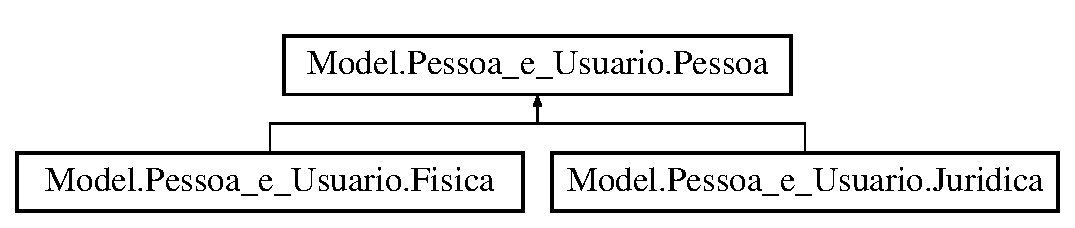
\includegraphics[height=2.000000cm]{class_model_1_1_pessoa__e___usuario_1_1_pessoa}
\end{center}
\end{figure}
\subsection*{Propriedades}
\begin{DoxyCompactItemize}
\item 
\hypertarget{class_model_1_1_pessoa__e___usuario_1_1_pessoa_a3be8ff18caae60ce0c42b1f513d1b3a3}{}string {\bfseries Nome}\hspace{0.3cm}{\ttfamily  \mbox{[}get, set\mbox{]}}\label{class_model_1_1_pessoa__e___usuario_1_1_pessoa_a3be8ff18caae60ce0c42b1f513d1b3a3}

\item 
\hypertarget{class_model_1_1_pessoa__e___usuario_1_1_pessoa_a003d71b706cf5b814ce35128b5a5a504}{}string {\bfseries Endereco}\hspace{0.3cm}{\ttfamily  \mbox{[}get, set\mbox{]}}\label{class_model_1_1_pessoa__e___usuario_1_1_pessoa_a003d71b706cf5b814ce35128b5a5a504}

\item 
\hypertarget{class_model_1_1_pessoa__e___usuario_1_1_pessoa_af62ae15131b638fb15bcc508a3f2ce48}{}string {\bfseries Email}\hspace{0.3cm}{\ttfamily  \mbox{[}get, set\mbox{]}}\label{class_model_1_1_pessoa__e___usuario_1_1_pessoa_af62ae15131b638fb15bcc508a3f2ce48}

\item 
\hypertarget{class_model_1_1_pessoa__e___usuario_1_1_pessoa_a8cf4fad5e567a3064265bf5acd5b320b}{}string {\bfseries Situacao}\hspace{0.3cm}{\ttfamily  \mbox{[}get, set\mbox{]}}\label{class_model_1_1_pessoa__e___usuario_1_1_pessoa_a8cf4fad5e567a3064265bf5acd5b320b}

\item 
\hypertarget{class_model_1_1_pessoa__e___usuario_1_1_pessoa_a90d0acb47aa0e92f8d4aad4f8d9e4dd5}{}string {\bfseries Sigla\+Estado}\hspace{0.3cm}{\ttfamily  \mbox{[}get, set\mbox{]}}\label{class_model_1_1_pessoa__e___usuario_1_1_pessoa_a90d0acb47aa0e92f8d4aad4f8d9e4dd5}

\item 
\hypertarget{class_model_1_1_pessoa__e___usuario_1_1_pessoa_ae0e926f4b8f9747616d9f07f1165775e}{}string {\bfseries Cidade}\hspace{0.3cm}{\ttfamily  \mbox{[}get, set\mbox{]}}\label{class_model_1_1_pessoa__e___usuario_1_1_pessoa_ae0e926f4b8f9747616d9f07f1165775e}

\item 
\hypertarget{class_model_1_1_pessoa__e___usuario_1_1_pessoa_af8a1663760e26d6d4e81ef310dfef97b}{}string {\bfseries Bairro}\hspace{0.3cm}{\ttfamily  \mbox{[}get, set\mbox{]}}\label{class_model_1_1_pessoa__e___usuario_1_1_pessoa_af8a1663760e26d6d4e81ef310dfef97b}

\item 
\hypertarget{class_model_1_1_pessoa__e___usuario_1_1_pessoa_a52bd778675e844d78867afa43018f7ad}{}string {\bfseries Cep}\hspace{0.3cm}{\ttfamily  \mbox{[}get, set\mbox{]}}\label{class_model_1_1_pessoa__e___usuario_1_1_pessoa_a52bd778675e844d78867afa43018f7ad}

\item 
\hypertarget{class_model_1_1_pessoa__e___usuario_1_1_pessoa_af6c352f8039298ee93e7efeb4427f945}{}string {\bfseries Observacoes}\hspace{0.3cm}{\ttfamily  \mbox{[}get, set\mbox{]}}\label{class_model_1_1_pessoa__e___usuario_1_1_pessoa_af6c352f8039298ee93e7efeb4427f945}

\end{DoxyCompactItemize}


A documentação para esta classe foi gerada a partir do seguinte ficheiro\+:\begin{DoxyCompactItemize}
\item 
C\+:/\+Cristiano/\+Projetos/\+Software\+Ordem\+De\+Servico/\+Model/\+Pessoa e Usuario/Pessoa.\+cs\end{DoxyCompactItemize}

\hypertarget{class_view_console_1_1_program}{}\section{Referência à classe View\+Console.\+Program}
\label{class_view_console_1_1_program}\index{View\+Console.\+Program@{View\+Console.\+Program}}


A documentação para esta classe foi gerada a partir do seguinte ficheiro\+:\begin{DoxyCompactItemize}
\item 
D\+:/\+Projetos/\+Software\+Ordem\+De\+Servico/\+View\+Console/Program.\+cs\end{DoxyCompactItemize}

\hypertarget{class_model_1_1_ordem__de___servico_1_1_servico}{}\section{Referência à classe Model.\+Ordem\+\_\+de\+\_\+\+Servico.\+Servico}
\label{class_model_1_1_ordem__de___servico_1_1_servico}\index{Model.\+Ordem\+\_\+de\+\_\+\+Servico.\+Servico@{Model.\+Ordem\+\_\+de\+\_\+\+Servico.\+Servico}}
\subsection*{Propriedades}
\begin{DoxyCompactItemize}
\item 
\hypertarget{class_model_1_1_ordem__de___servico_1_1_servico_a094d3e4aa689cb0c8df45206b7f1a5fc}{}string {\bfseries Descricao}\hspace{0.3cm}{\ttfamily  \mbox{[}get, set\mbox{]}}\label{class_model_1_1_ordem__de___servico_1_1_servico_a094d3e4aa689cb0c8df45206b7f1a5fc}

\item 
\hypertarget{class_model_1_1_ordem__de___servico_1_1_servico_a54366b1a10051d3df2084aaa14691643}{}double {\bfseries Valor}\hspace{0.3cm}{\ttfamily  \mbox{[}get, set\mbox{]}}\label{class_model_1_1_ordem__de___servico_1_1_servico_a54366b1a10051d3df2084aaa14691643}

\end{DoxyCompactItemize}


A documentação para esta classe foi gerada a partir do seguinte ficheiro\+:\begin{DoxyCompactItemize}
\item 
D\+:/\+Projetos/\+Software\+Ordem\+De\+Servico/\+Model/\+Ordem de Servico/Servico.\+cs\end{DoxyCompactItemize}

\hypertarget{class_model_1_1_pessoa__e___usuario_1_1_usuario}{}\section{Referência à classe Model.\+Pessoa\+\_\+e\+\_\+\+Usuario.\+Usuario}
\label{class_model_1_1_pessoa__e___usuario_1_1_usuario}\index{Model.\+Pessoa\+\_\+e\+\_\+\+Usuario.\+Usuario@{Model.\+Pessoa\+\_\+e\+\_\+\+Usuario.\+Usuario}}
\subsection*{Membros públicos}
\begin{DoxyCompactItemize}
\item 
String \hyperlink{class_model_1_1_pessoa__e___usuario_1_1_usuario_a7904f8842d9978778f7ab375dac1598a}{Save} (String \+\_\+\+Nome, String \+\_\+\+Senha, string \+\_\+\+Nivel\+Acesso)
\begin{DoxyCompactList}\small\item\em Salvando novo usuário \end{DoxyCompactList}\item 
List$<$ string $>$ \hyperlink{class_model_1_1_pessoa__e___usuario_1_1_usuario_aaafe59d54bd44b2cd36f9b7032df5ba3}{Load\+List} ()
\begin{DoxyCompactList}\small\item\em Carregando Lista com nome de todos usuarios. \end{DoxyCompactList}\item 
\hyperlink{class_model_1_1_pessoa__e___usuario_1_1_usuario}{Usuario} \hyperlink{class_model_1_1_pessoa__e___usuario_1_1_usuario_ab5b4ff8011ebf25cddea82c55ca7cb4e}{Load} (string \+\_\+\+Nome)
\begin{DoxyCompactList}\small\item\em Carregando usuario. \end{DoxyCompactList}\item 
bool \hyperlink{class_model_1_1_pessoa__e___usuario_1_1_usuario_aafad0b4e2f96cc058b92033da5dcb193}{Verificar} (string \+\_\+nome)
\begin{DoxyCompactList}\small\item\em Verificando de o suario existe. \end{DoxyCompactList}\end{DoxyCompactItemize}
\subsection*{Propriedades}
\begin{DoxyCompactItemize}
\item 
\hypertarget{class_model_1_1_pessoa__e___usuario_1_1_usuario_ab28403069bfa081c90c4570139e1c923}{}string {\bfseries Nome}\hspace{0.3cm}{\ttfamily  \mbox{[}get, set\mbox{]}}\label{class_model_1_1_pessoa__e___usuario_1_1_usuario_ab28403069bfa081c90c4570139e1c923}

\item 
\hypertarget{class_model_1_1_pessoa__e___usuario_1_1_usuario_a6a111adad476bc88b0320febd535e170}{}string {\bfseries Senha}\hspace{0.3cm}{\ttfamily  \mbox{[}get, set\mbox{]}}\label{class_model_1_1_pessoa__e___usuario_1_1_usuario_a6a111adad476bc88b0320febd535e170}

\item 
\hypertarget{class_model_1_1_pessoa__e___usuario_1_1_usuario_a57734a8566a6930b043bcaae24aae066}{}string {\bfseries Nivel\+Acesso}\hspace{0.3cm}{\ttfamily  \mbox{[}get, set\mbox{]}}\label{class_model_1_1_pessoa__e___usuario_1_1_usuario_a57734a8566a6930b043bcaae24aae066}

\end{DoxyCompactItemize}


\subsection{Documentação dos métodos}
\hypertarget{class_model_1_1_pessoa__e___usuario_1_1_usuario_ab5b4ff8011ebf25cddea82c55ca7cb4e}{}\index{Model\+::\+Pessoa\+\_\+e\+\_\+\+Usuario\+::\+Usuario@{Model\+::\+Pessoa\+\_\+e\+\_\+\+Usuario\+::\+Usuario}!Load@{Load}}
\index{Load@{Load}!Model\+::\+Pessoa\+\_\+e\+\_\+\+Usuario\+::\+Usuario@{Model\+::\+Pessoa\+\_\+e\+\_\+\+Usuario\+::\+Usuario}}
\subsubsection[{Load(string \+\_\+\+Nome)}]{\setlength{\rightskip}{0pt plus 5cm}{\bf Usuario} Model.\+Pessoa\+\_\+e\+\_\+\+Usuario.\+Usuario.\+Load (
\begin{DoxyParamCaption}
\item[{string}]{\+\_\+\+Nome}
\end{DoxyParamCaption}
)}\label{class_model_1_1_pessoa__e___usuario_1_1_usuario_ab5b4ff8011ebf25cddea82c55ca7cb4e}


Carregando usuario. 


\begin{DoxyParams}{Parâmetros}
{\em \+\_\+\+Nome} & \\
\hline
\end{DoxyParams}
\begin{DoxyReturn}{Retorna}
\hyperlink{class_model_1_1_pessoa__e___usuario_1_1_usuario}{Usuario}
\end{DoxyReturn}
\hypertarget{class_model_1_1_pessoa__e___usuario_1_1_usuario_aaafe59d54bd44b2cd36f9b7032df5ba3}{}\index{Model\+::\+Pessoa\+\_\+e\+\_\+\+Usuario\+::\+Usuario@{Model\+::\+Pessoa\+\_\+e\+\_\+\+Usuario\+::\+Usuario}!Load\+List@{Load\+List}}
\index{Load\+List@{Load\+List}!Model\+::\+Pessoa\+\_\+e\+\_\+\+Usuario\+::\+Usuario@{Model\+::\+Pessoa\+\_\+e\+\_\+\+Usuario\+::\+Usuario}}
\subsubsection[{Load\+List()}]{\setlength{\rightskip}{0pt plus 5cm}List$<$string$>$ Model.\+Pessoa\+\_\+e\+\_\+\+Usuario.\+Usuario.\+Load\+List (
\begin{DoxyParamCaption}
{}
\end{DoxyParamCaption}
)}\label{class_model_1_1_pessoa__e___usuario_1_1_usuario_aaafe59d54bd44b2cd36f9b7032df5ba3}


Carregando Lista com nome de todos usuarios. 

\begin{DoxyReturn}{Retorna}

\end{DoxyReturn}
\hypertarget{class_model_1_1_pessoa__e___usuario_1_1_usuario_a7904f8842d9978778f7ab375dac1598a}{}\index{Model\+::\+Pessoa\+\_\+e\+\_\+\+Usuario\+::\+Usuario@{Model\+::\+Pessoa\+\_\+e\+\_\+\+Usuario\+::\+Usuario}!Save@{Save}}
\index{Save@{Save}!Model\+::\+Pessoa\+\_\+e\+\_\+\+Usuario\+::\+Usuario@{Model\+::\+Pessoa\+\_\+e\+\_\+\+Usuario\+::\+Usuario}}
\subsubsection[{Save(\+String \+\_\+\+Nome, String \+\_\+\+Senha, string \+\_\+\+Nivel\+Acesso)}]{\setlength{\rightskip}{0pt plus 5cm}String Model.\+Pessoa\+\_\+e\+\_\+\+Usuario.\+Usuario.\+Save (
\begin{DoxyParamCaption}
\item[{String}]{\+\_\+\+Nome, }
\item[{String}]{\+\_\+\+Senha, }
\item[{string}]{\+\_\+\+Nivel\+Acesso}
\end{DoxyParamCaption}
)}\label{class_model_1_1_pessoa__e___usuario_1_1_usuario_a7904f8842d9978778f7ab375dac1598a}


Salvando novo usuário 


\begin{DoxyParams}{Parâmetros}
{\em \+\_\+\+Nome} & \\
\hline
{\em \+\_\+\+Senha} & \\
\hline
{\em \+\_\+\+Nivel\+Acesso} & \\
\hline
\end{DoxyParams}
\begin{DoxyReturn}{Retorna}

\end{DoxyReturn}
\hypertarget{class_model_1_1_pessoa__e___usuario_1_1_usuario_aafad0b4e2f96cc058b92033da5dcb193}{}\index{Model\+::\+Pessoa\+\_\+e\+\_\+\+Usuario\+::\+Usuario@{Model\+::\+Pessoa\+\_\+e\+\_\+\+Usuario\+::\+Usuario}!Verificar@{Verificar}}
\index{Verificar@{Verificar}!Model\+::\+Pessoa\+\_\+e\+\_\+\+Usuario\+::\+Usuario@{Model\+::\+Pessoa\+\_\+e\+\_\+\+Usuario\+::\+Usuario}}
\subsubsection[{Verificar(string \+\_\+nome)}]{\setlength{\rightskip}{0pt plus 5cm}bool Model.\+Pessoa\+\_\+e\+\_\+\+Usuario.\+Usuario.\+Verificar (
\begin{DoxyParamCaption}
\item[{string}]{\+\_\+nome}
\end{DoxyParamCaption}
)}\label{class_model_1_1_pessoa__e___usuario_1_1_usuario_aafad0b4e2f96cc058b92033da5dcb193}


Verificando de o suario existe. 


\begin{DoxyParams}{Parâmetros}
{\em \+\_\+nome} & \\
\hline
\end{DoxyParams}
\begin{DoxyReturn}{Retorna}

\end{DoxyReturn}


A documentação para esta classe foi gerada a partir do seguinte ficheiro\+:\begin{DoxyCompactItemize}
\item 
D\+:/\+Projetos/\+Software\+Ordem\+De\+Servico/\+Model/\+Pessoa e Usuario/Usuario.\+cs\end{DoxyCompactItemize}

%--- End generated contents ---

% Index
\backmatter
\newpage
\phantomsection
\clearemptydoublepage
\addcontentsline{toc}{chapter}{Índice}
\printindex

\end{document}
